\newpage
\setcounter{subsection}{0}
%Change formatting for tis section

\titleformat{\section}[frame]
{\fontsize{24pt}{28.8pt}\selectfont\bfseries} {} {5pt} {}
\titleformat{\subsection}[display]
{\fontsize{18pt}{21.6pt}\selectfont\bfseries} {} {5pt} {\thesubsection\quad}
\titleformat{\subsubsection}[display]
{\fontsize{14pt}{16.8pt}\selectfont\bfseries} {} {5pt} {\thesubsubsection\quad}
\renewcommand\thesubsection{\arabic{subsection}.}
\renewcommand\thesubsubsection{\arabic{subsection}.\arabic{subsubsection}}
\rhead{\rightmark}
%add paragraph as extra level for experiments
\setcounter{secnumdepth}{5}
\titleformat{\paragraph}[display]
{\fontsize{12pt}{14pt}\selectfont\bfseries}{}{5pt} {\theparagraph\quad}
%add subparagraph
\titleformat{\subparagraph}[display]
{\fontsize{12pt}{14pt}}{}{5pt} {\thesubparagraph\quad}
\renewcommand\thesubparagraph{\arabic{subsection}.\arabic{subsubsection}.\arabic{paragraph}\alph{subparagraph}}


%Start
\section*{Part 4. Main report}
\addcontentsline{toc}{section}{Part 4. Main report}
\markright{Part 4. Main report}
\secun{Literature study}
\pagenumbering{arabic}
\captionsetup[table]{position=bottom}
\subsubsection{Background and context}

\subsubsection{Application of background to this project}
In this section of the report, a brief overview of the existing research that is relevant to this project will be given, as well as a short discussion on how this existing research will be used to aid in the design of a five legged holonomic robot during the course of this project.\\

Legged vehicles are preferred to wheeled vehicles for exploration and rescue in remote areas because of their ability to cross rough terrain quickly with a severely reduced risk of getting stuck. The price to pay for this superior drive-train is far more complex electronics and movement algorithms \cite{Hidayat:Autonomous}. Instead of just driving the wheel motors and steering, each limb actuator of each leg has to be controlled to move to a calculated position.\\ 

Inverse kinematics is the mathematical process used to calculate the required angles of the limbs of a structure to reach a specific set of coordinates. This is used extensively in this project because of its ability to easily transform desired Cartesian coordinates into the required actuator angles. In the paper \cite{Oh:Analytic}, a method is discussed for solving the inverse kinematic equations involved in a seven degrees of freedom robotic arm. This method takes into account specified minimum and maximum values for each actuator and degree of freedom in order to avoid self-collision. This method can be applied to any system with a specified degrees of freedom and can therefore be simplified to solve the inverse kinematic equations for the system designed in this project.\\

To obtain the Cartesian coordinates desired at any given time, the method described in \cite{Hidayat:Autonomous}, namely Sine pattern methods is used. In \cite{Hidayat:Autonomous}, the method was applied to a quadruped robot. In the case of this project, the method is expanded to make it suitable for use on a robot with five legs. Adaptation is required because the method relies on the symmetry of a quadruped robot to schedule the lifting of the legs. Since the same symmetry does not exist in a robot with five legs, a different scheduling technique is investigated. This method will rely on information from the current position of the legs, the limits of leg movement, as well as the current horizontal tilt of the robot.\\

In the conference paper \cite{Jain:Odometry}, motion planning of omnidirectional robots is discussed and a sophisticated yet simple and efficient method of route planning is proposed. This method is based on vehicles that use three omnidirectional wheels in combination to form a resultant force vector in the desired direction. These type of vehicles differ largely in terms of locomotion when compared to the holonomic legged design used in this project, but there are a few key similarities. Both these designs can move holonomically, therefore they have the ability to move in a straight line while rotating, move in an arc without rotating, or any combination of the two. These similarities mean that some of the methods discussed and applied in \cite{Jain:Odometry} can be used to aid in the design of the algorithm used in this project.\\

A team from Instituto Tecnologico de la Laguna in Mexico designed a hexapod robot \cite{Ollervides:Navigation} similar to the robot designed in this project. The purpose of the hexapod was to investigate its potential for use in exploration of areas that are hard to reach by any commonly used means of transportation. Legged vehicles are more suited to cross rough terrain, but rough terrain complicates the design of the drive-train. In applications where the surface is smooth or close to smooth, open loop control can be applied where the leg is simply moved to the desired position and it is assumed by the designer that the robot foot is making contact with the ground at this point, and therefore supporting part of the distributed robot weight. When the robot is crossing rough terrain, where the surface consists of mainly bumps and holes, this assumption could be false. In such a scenario, the robot could lift another leg while under the impression that its weight is being supported by the other legs. If this is not the case, the robot could fall over and possibly damage itself or be unable to rectify itself. To avoid this problem, closed loop control should be used in the height positioning of the legs. This involves having a sensor in the system that could provide feedback on the state of the foot. The hexapod in \cite{Ollervides:Navigation} used miniature resistive force sensors attached to the bottom of each foot of the robot. The robot therefore has the ability to take analogue measurements from these sensors and determine the weight distribution of the individual feet of the robot. This data is used to confirm that all robot feet are making contact with the surface and correct the situation if this is not the case. This type of feedback is also useful when the robot is operated on slanted surfaces because of the effect that the center of gravity has on a slanted surface. A feedback sensor will be included in the design of the five legged holonomic robot in this project.\\

If the robot is operating on a slanted surface without it being aware of this and the centre of gravity shifts over the lowest foot making contact, the robot could fall over even when all of its legs are making contact with the surface. In a paper on reactive robot navigation \cite{Arkin:Reactive}, it is proposed that the use of a digital inclinometer can aid in solving this problem. The sensor provides information on the current tilt of the robot in two dimensions. This sensor in combination with the feedback sensors on the robot feet can be used to ensure that the robot levels itself automatically to avoid tipping over. The data collected from this sensor can also be used to collect information on the terrain. In the journal article \cite{Arkin:Reactive}, this data is used for hill climbing as well as finding valleys in unexplored areas. In order to enable the robot designed in this project to walk on slanted surfaces, a digital inclinometer will be used. Some of the reactive navigation techniques discussed in \cite{Arkin:Reactive} will also be implemented to aid the robot in navigating on slanted planes.\\

In a paper on the effects of slippery surfaces on biped robots \cite{Hyeon:Reflex}, methods on avoiding falling over of a biped robot is investigated. Since these robots have to balance themselves to stay upright, an unforeseen slippery patch on a surface could be fatal for the robot. If it were possible to foresee a slippery surface, slowing down the walking gait and increasing foot surface would help increase the traction of the robot, and therefore lower the risk of slipping. Since a five legged robot is inherently stable and there is no balancing required, slippery surfaces may influence the traction of the robot but there is very low risk of falling over on level surfaces that are slippery. It is therefore suitable to just slow down movements on slippery surfaces to increase the traction where possible.

\secun{Approach}
This section outlines the initial approach to solve the functions shown in the functional block diagram. The functional block diagram of the project can be found in Figure \ref{fig:Func}
\subsubsection{Design alternatives}

\subsubsection{Preferred solution}



\secun{Design and implementation}
\subsubsection{Background}
A large part of the design of a legged robot depends on the design of a simple leg - more specifically the degrees of freedom that a single leg has. The degrees of freedom that a single leg has is determined by the amount of dimensions that the leg can make a controlled movement in, independently from any other dimensions. There are two common underlying designs in robot leg design - these are for two and three degrees of freedom respectively.\\

Figure \ref{fig:2DOF} shows an example of a common design that has two degrees of freedom. The design therefore contains two joints in one leg. In this example, the first joint is positioned vertically to form the hip op the robot leg. This allows for the side-to-side motion required for walking. The second joint is positioned horizontally to allow the lowest limb to move up and down. The two degrees of freedom controlled by this leg design is therefore the horizontal angle of the leg and the height of the foot. These two (and only these two) parameters can therefore be controlled completely independently.
\FloatBarrier
\begin{figure}[h]
\centering
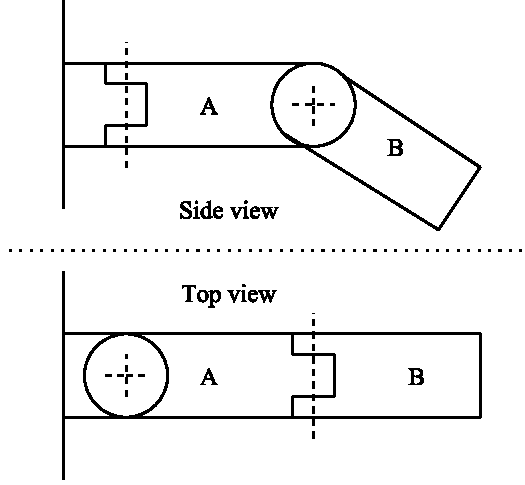
\includegraphics[scale = 1]{pics/2DOF.pdf}
\caption{Example of a leg design with two degrees of freedom.}
\label{fig:2DOF}
\end{figure}
\FloatBarrier
An example of a robotic leg with three degrees of freedom can be seen in Figure \ref{fig:3DOF}. This design is similar to that of the leg with two degrees of freedom seen in Figure \ref{fig:2DOF}, with the only addition being a second horizontal joint further down from the first. This additional limb means that the horizontal distance from the foot to the hip can be controlled as well as the height of the foot. These two controlled parameters, together with the horizontal leg angle which can also be controlled independently as in the case of the two degrees of freedom design, means that this design has a total of three degrees of freedom.
\FloatBarrier
\begin{figure}[h]
\centering
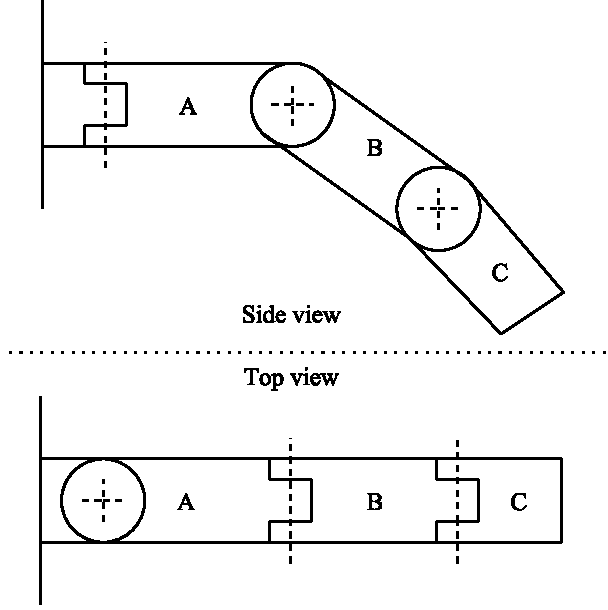
\includegraphics[scale = 1]{pics/3DOF.pdf}
\caption{Example of a leg design with three degrees of freedom.}
\label{fig:3DOF}
\end{figure}
\FloatBarrier


The design with three degrees of freedom has the advantage of being able to lift a leg without altering the horizontal position of the leg. This means that the robot is able to walk without altering the height of the body of the robot. The robot is therefore able to cross rougher terrain much better because of the ability to alter the height of the robot feet as the terrain requires. With the design that has two degrees of freedom, the foot height is a function of the horizontal extension of the leg. With this design the main advantage is the simplicity - both mechanically and in software. The cost and power consumption will also be much lower because of the reduced amount of actuators.\\

Due to the much greater flexibility of the design with three degrees of freedom and the ability to cross rougher terrain, this will be the platform implemented in the final design.\\

\subsubsection{Theoretical analysis and modelling}
\FloatBarrier
\begin{figure}[h]
\centering
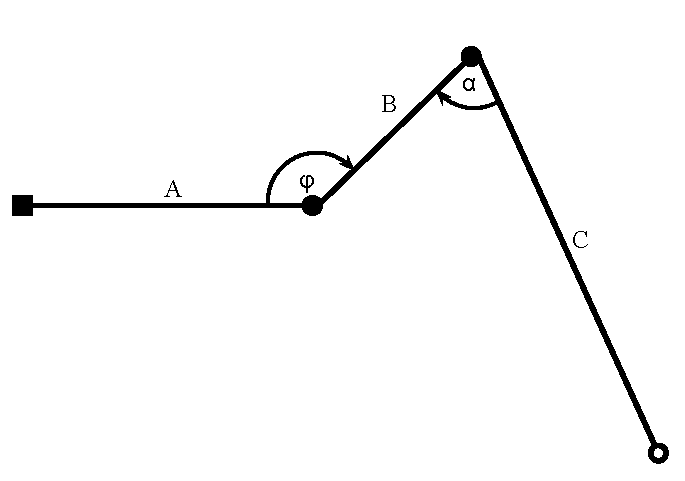
\includegraphics[scale = 1]{pics/Leg_design.pdf}
\caption{Simulation results for the network.}
\label{fig:Leg_design}
\end{figure}
\FloatBarrier

\FloatBarrier
\begin{figure}[h]
\centering
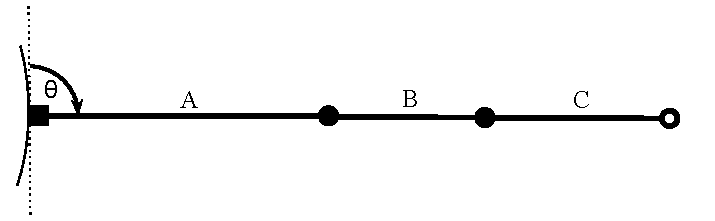
\includegraphics[scale = 1]{pics/Leg_design_2.pdf}
\caption{Simulation results for the network.}
\label{fig:Leg_design}
\end{figure}
\FloatBarrier

\subsubsection{Simulation}
\label{sec:sim}
In order to test the equations and design outlined in the Theory section above, the mathematics was implemented in a script written in the Python programming language and developed in the PyCharm IDE. The program consists of a GUI  used to enter elementary commands, similar to that implemented in the Android application, as well as a window for plotting the result in a 3-dimensional Cartesian system. Some results showing the validity of the design equations in the previous section can be found below. All of the source code used to build this simulation can be found in Part 5 of this report on the attached optical disc.\\

The program flow of the software in the simulation is similar to that used for the final prototype software, more information on the software design flow can be found in Section \ref{sec:soft}. The main difference between the final implementation and the simulation is that once the angle values for theta, alpha and phi are calculated for each leg, in the final implementation the result is used to move the actuator while in simulation the result is used to calculate the Cartesian position of each limb in order to plot it in the 3-dimensional system. It should be noted that the length of all of the limbs as well as the robot body radius was chosen as unity for simplicity and since the purpose of the simulation is only to show the functionality of the IK. It should also be noted that although some of the legs may look crooked in the following figures, this is only a result of the viewing angle. When viewed directly from above, all limbs of a single leg align in an upright plane.\\

The basic user interface together with the Robot in its neutral position can be seen in Figure \ref{fig:Sim1}.\\

The orange markers found at each of the robot feet indicate the neutral position for each of the five feet. This is indicated to aid in showing the movement of the legs relative to this neutral position in Figure \ref{fig:Sim1} and the figures following in this section.\\

\begin{figure}[H]
\centering
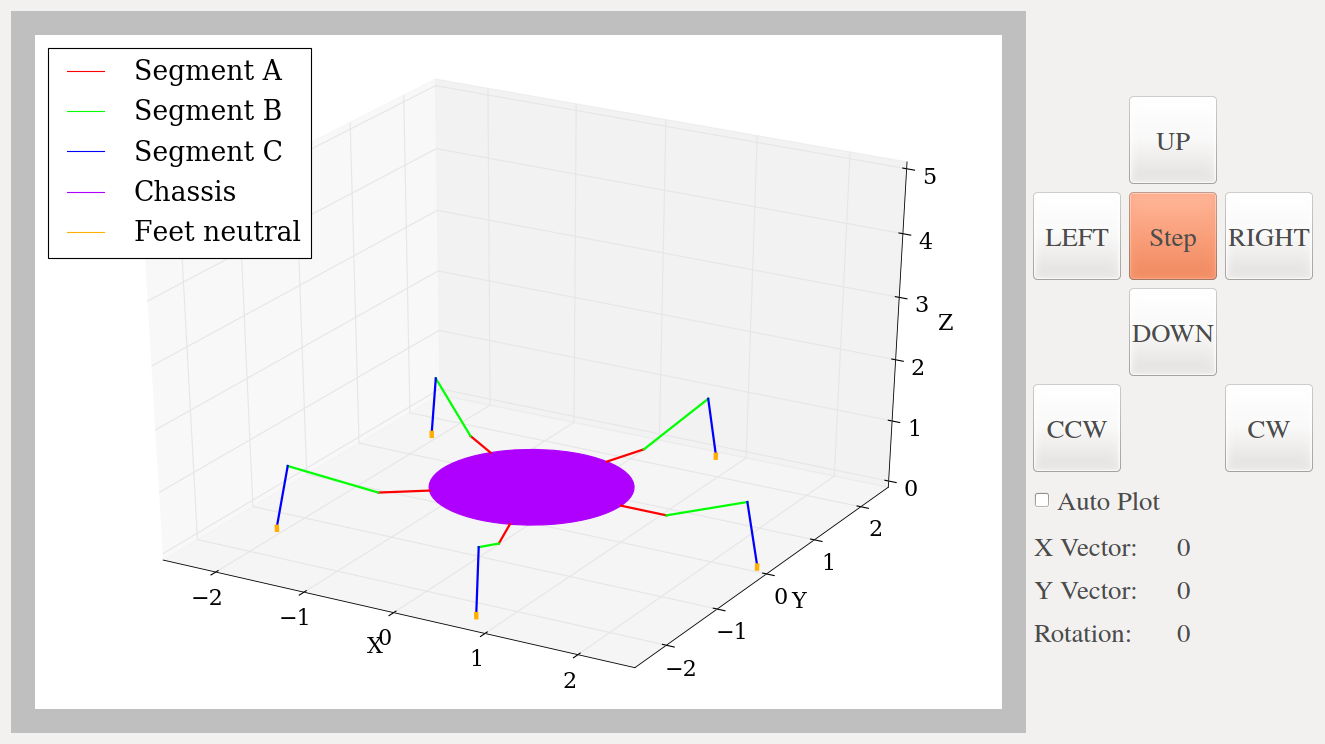
\includegraphics[scale = 0.33]{pics/Sim1.png}
\caption{Simulation window showing the robot in its neutral position.}
\label{fig:Sim1}
\end{figure}

When the $Y$ vector is changed to a positive value, the legs will all move in a negative $Y$-direction since the robot center is the origin. When the robot should move in a specific direction, the feet will move in the exact opposite direction to propel the robot forward. This is illustrated in Figure \ref{fig:Sim2}.

\begin{figure}[H]
\centering
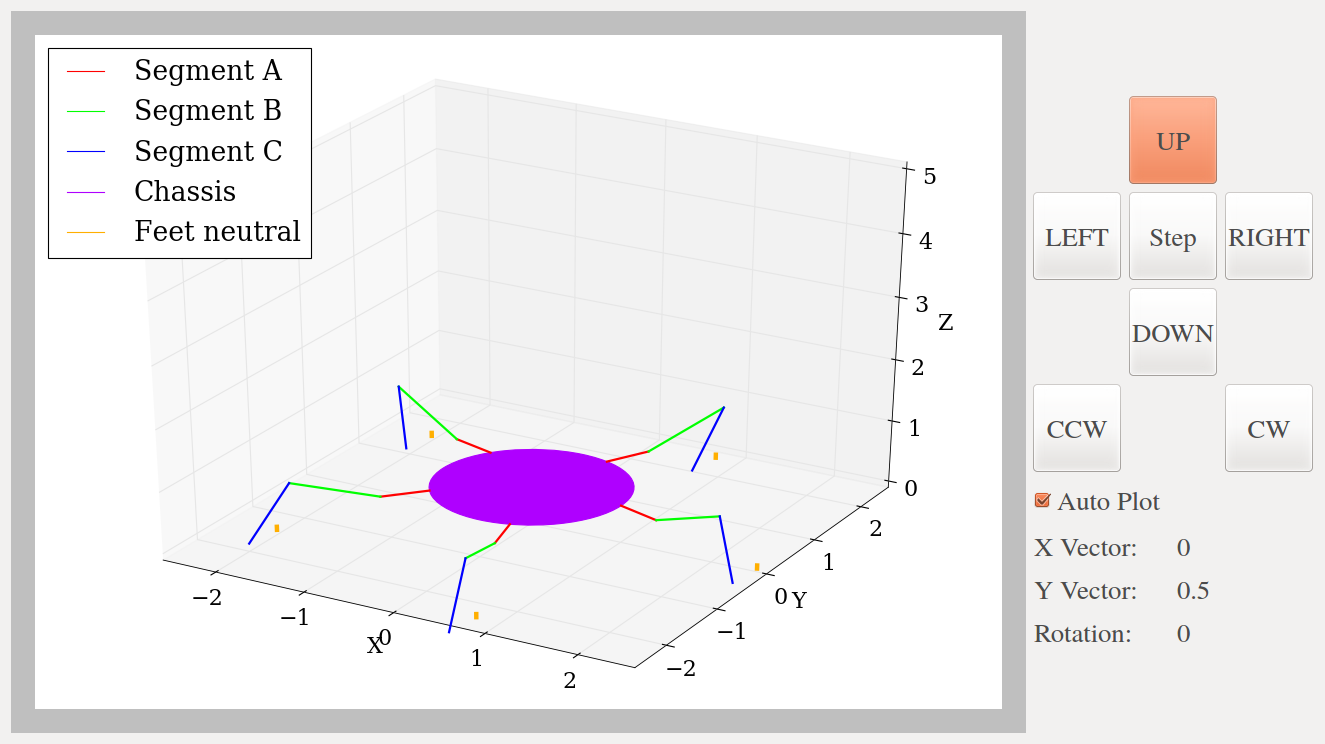
\includegraphics[scale = 0.33]{pics/Sim2.png}
\caption{Simulation window showing the robot moving in a positive $Y$-direction.}
\label{fig:Sim2}
\end{figure}

The robot should also be able to translate in the $X$-direction without making a rotation first. This is illustrated in Figure \ref{fig:Sim3}.

\begin{figure}[H]
\centering
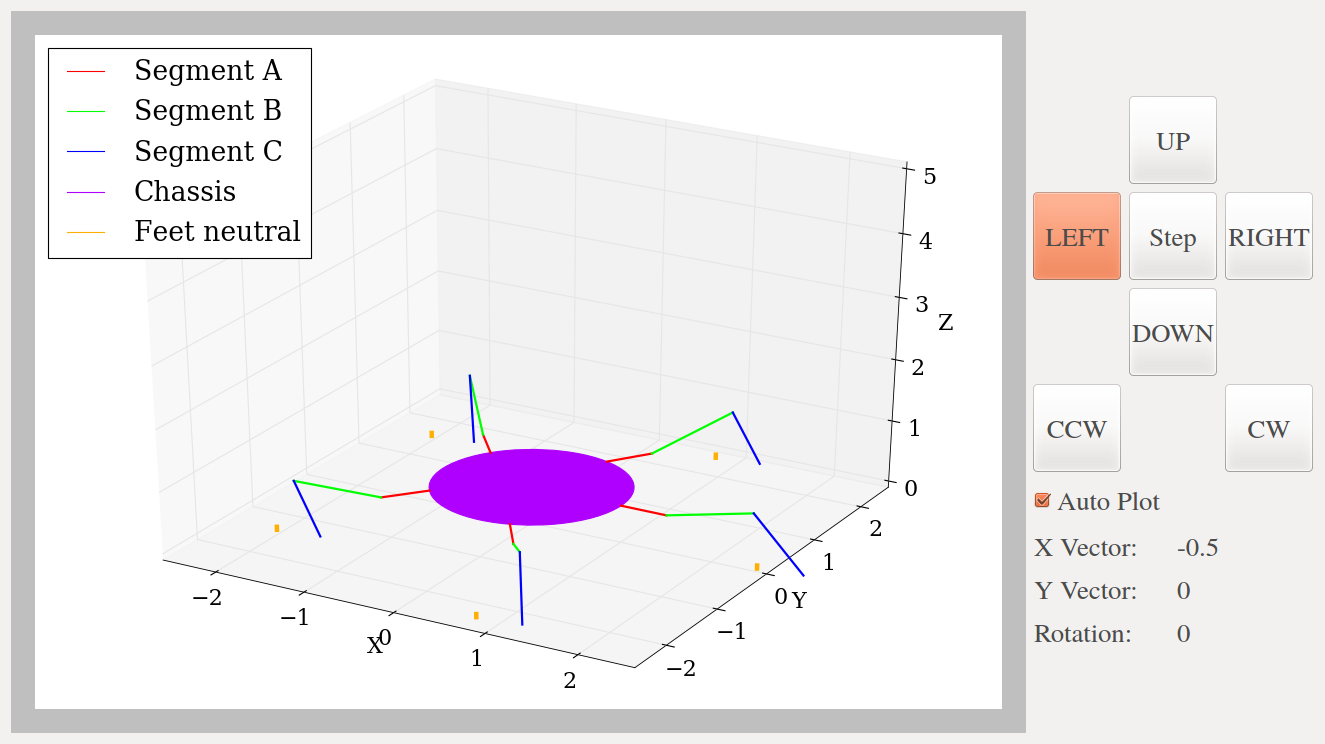
\includegraphics[scale = 0.33]{pics/Sim3.png}
\caption{Simulation window showing the robot moving in a negative $X$-direction.}
\label{fig:Sim3}
\end{figure}

If the robot can instantaneously move in both the $X$ and $Y$-directions, it should be able to move in a combination of the two without a problem. This ability is illustrated in Figure \ref{fig:Sim4}.

\begin{figure}[H]
\centering
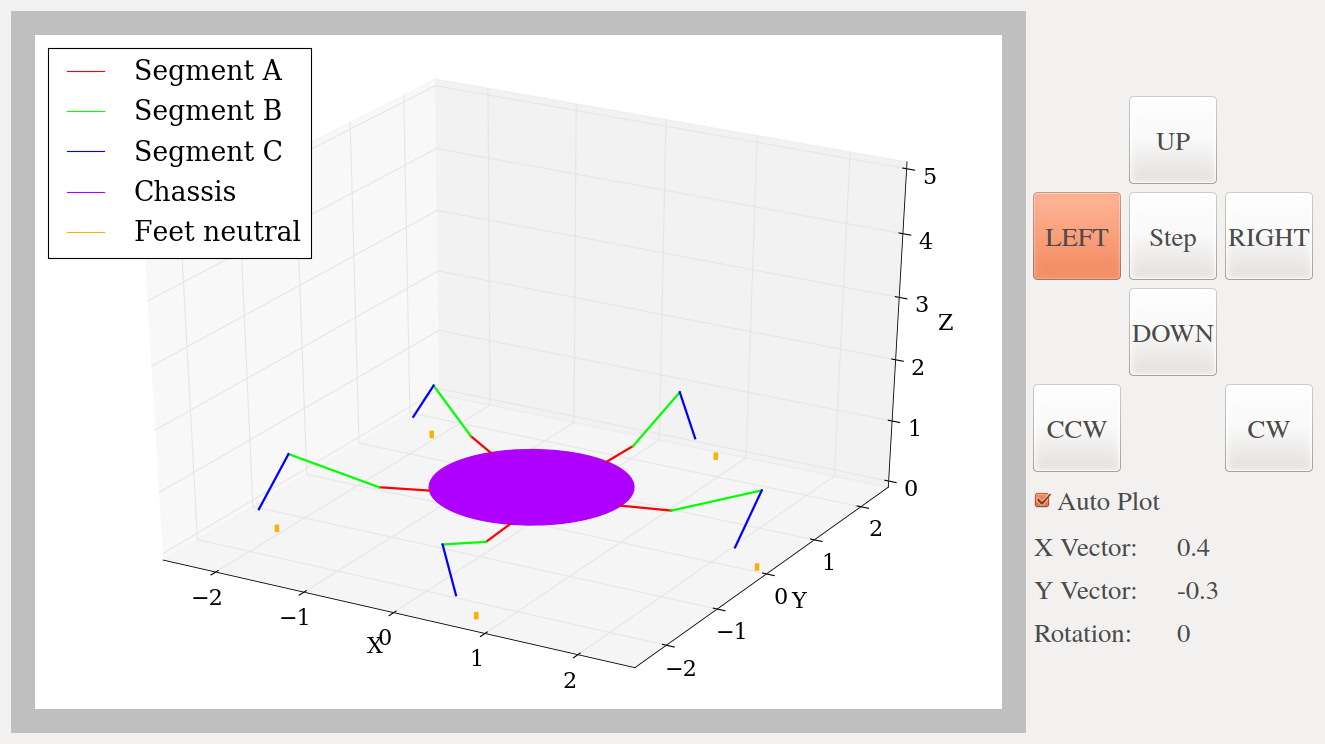
\includegraphics[scale = 0.33]{pics/Sim4.png}
\caption{Simulation window showing the robot moving in a direction with a positive $X$ and negative $Y$-component.}
\label{fig:Sim4}
\end{figure}

The translation appears to be working exactly as intended and designed for. The simulation is tested with a clockwise direction rotation in Figure \ref{fig:Sim5}.

\begin{figure}[H]
\centering
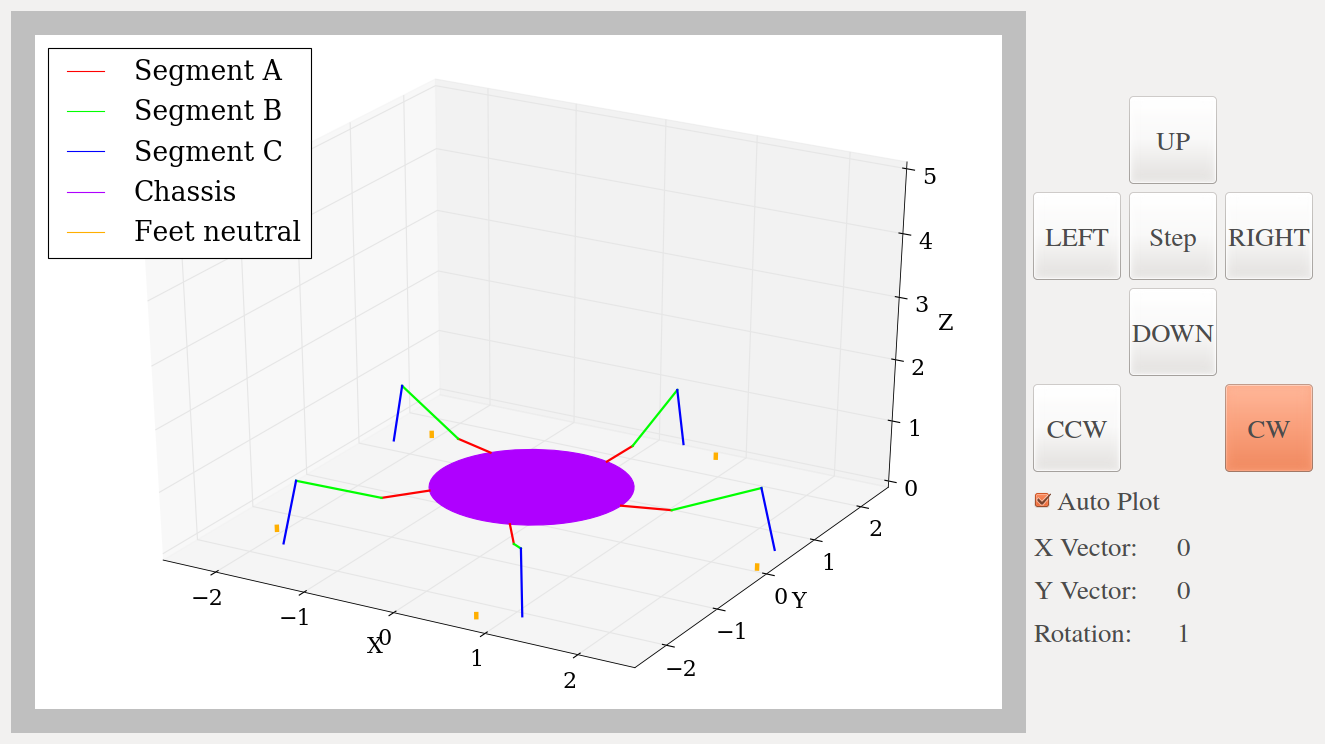
\includegraphics[scale = 0.33]{pics/Sim5.png}
\caption{Simulation window showing the robot rotating in a clockwise direction.}
\label{fig:Sim5}
\end{figure}

Once the robot reaches the boundary illustrated in Figure \ref{fig:Body_layout_3} for any of its legs, it is necessary to lift the leg up, move it to a more suitable location and put it down in order to continue in the direction it is heading in. This ability is illustrated in Figure \ref{fig:Sim6}.

\begin{figure}[H]
\centering
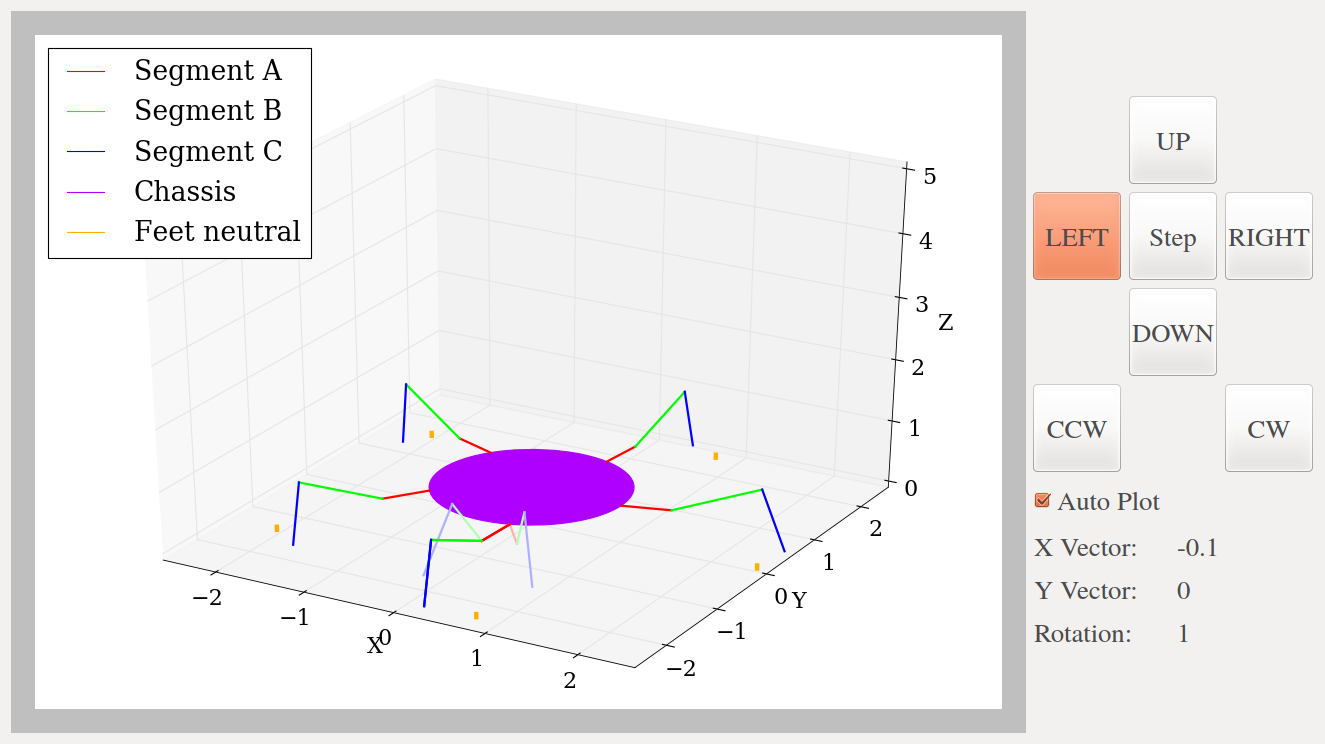
\includegraphics[scale = 0.33]{pics/Sim6.png}
\caption{Simulation window showing the robot picking up a foot and placing it again.}
\label{fig:Sim6}
\end{figure}

In Figure \ref{fig:Sim6}, the closest leg appears three times, twice in dimmed (ghost) colours and then finally in the normal colours. What this attempts to illustrate is the resetting motion of the leg. Figure \ref{fig:Sim5} shows the robot just before the resetting action. The right of the two "ghost" legs is right above the original location of the leg. This shows the position of the leg after it was lifted up. The left of the two "ghost" legs is the leg, still lifted, after being moved to a position directly over the new location. The leg plotted in full colour shows the final position of the leg. It is now able to start rotating further in the clockwise direction. Th robot will pickup and replace one leg at a time for all the legs that requires resetting and then continue.


\subsubsection{Optimisation}
The design of the algorithm used in the simulation works very well to systematically determine the 15 required servo angles. This is done from the three input values $(X,Y,R)$ which ultimately represent the speed for the $X$-direction, $Y$-direction and Rotation. What the simulation fails to take into account is the practical time constraints necessary to make a robot work. In simulation the result was just plotted so all the movement could be done instantaneously. In practice, however, the servo motors used to control the limbs of the robot need time to adjust to the set position. These servo motors use traditional analogue proportional, integral, derivative (PID) control techniques. The derivative term means that a sudden, large change in setpoint would result in a large current surge as a result of the PID controller trying to get to the setpoint as soon as possible. If all 15 of the servo motors are updated at the same time with a large jump in position, the surge in current required from each individual servo motor would sum to a large surge, possibly causing a brief dip in the system voltage. The solution to this is to not make large changes in setpoint between updates to the servo motors, but rather smaller updates more frequently. The exact time between updates will be a function of a how long it takes the floating point arithmetic (FPU) unit of the microcontroller to do all the floating point math required by the IK algorithm once.

%Electronics
\subsubsection{Electronic design}

\subsubsection{Electronic implementation}

\captionsetup[table]{position=bottom}
%Software
\subsubsection{Software design}
\label{sec:soft}

\subsubsection{Software implementation}
%Hardware
\subsubsection{Hardware design}
This section covers the design of all of the mechanical hardware that was designed specifically for this project.\\

The first of the parts to be designed were the legs, this would determine the scale of the robot. The legs were designed in three different segments as discussed in the theoretical and mathematical analysis. In order to simplify the mechanical design and distribute the weight of the robot more evenly, the servos are mounted inside the legs. Because the legs are lifted by the servos, these should be as close as possible to the hip in order to minimize the leverage on the servo lifting the leg.\\

The annotations in Figure \ref{fig:DrawingA} that shows segment A is explained below:
\begin{enumerate}
\item Gear that connects to the servo motor located in leg B.
\item Hole for wire management.
\item Gear teeth that connect to the servo motor located in the base.
\item Centreline where a stainless steel shaft is inserted into bearings for horizontal movement.
\item Centreline where a stainless steel shaft is inserted into bearings for vertical movement.
\end{enumerate}

\begin{figure}[H]
\centering
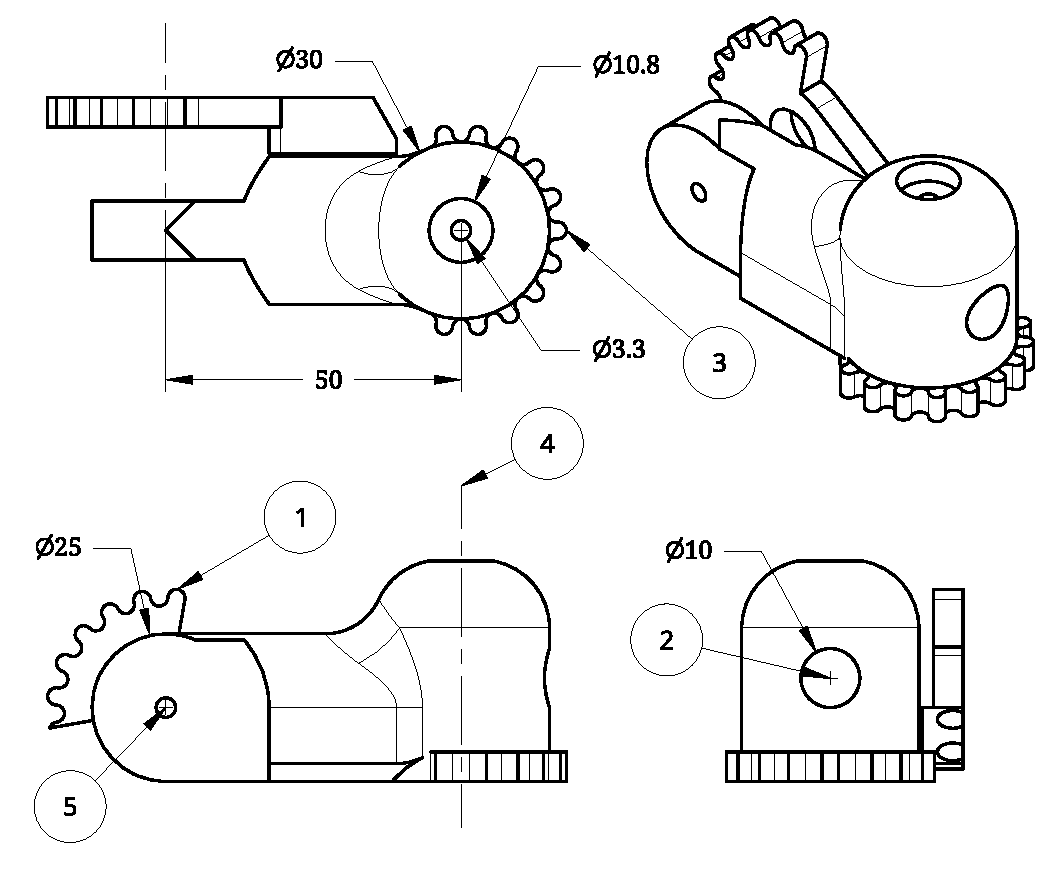
\includegraphics[scale = 0.8]{pics/DrawingA.pdf}
\caption{Illustration of how multiple servo motors are controlled using two timers.}
\label{fig:DrawingA}
\end{figure}

The annotations in Figure \ref{fig:DrawingB} that shows segment B is explained below:
\begin{enumerate}
\item Cavity for the servo motor that drives segment C.
\item Cavity for the servo motor that drives segment B.
\item Ball with slot that connects to segment A.
\item Peg that goes in the ball with slot in segment C.
\item Centreline where a stainless steel shaft is inserted into bearings for vertical movement with segment C.
\item Centreline where a stainless steel shaft is inserted into bearings for vertical movement with segment A.
\end{enumerate}

\begin{figure}[H]
\centering
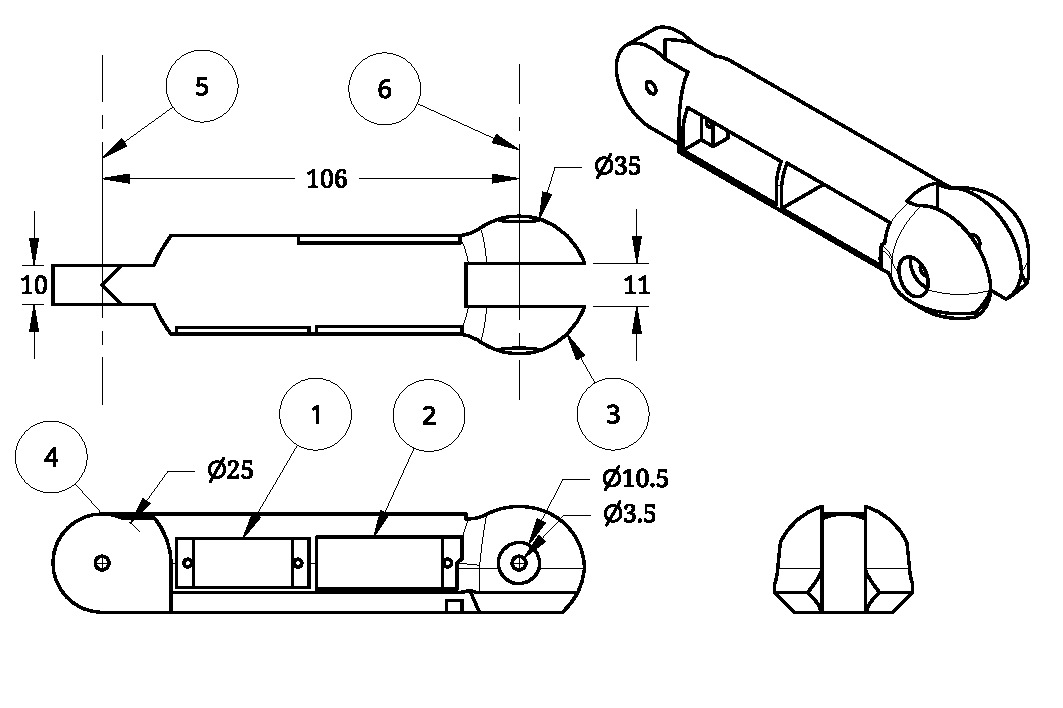
\includegraphics[scale = 0.8]{pics/DrawingB.pdf}
\caption{Illustration of how multiple servo motors are controlled using two timers.}
\label{fig:DrawingB}
\end{figure}

The annotations in Figure \ref{fig:DrawingC} that shows segment C is explained below:
\begin{enumerate}
\item Centreline where a stainless steel shaft is inserted into bearings for vertical movement with segment B.
\item Flat part of the foot that makes contact with the ground.
\item Cut-out that allows for a wider range of movement.
\end{enumerate}

\begin{figure}[H]
\centering
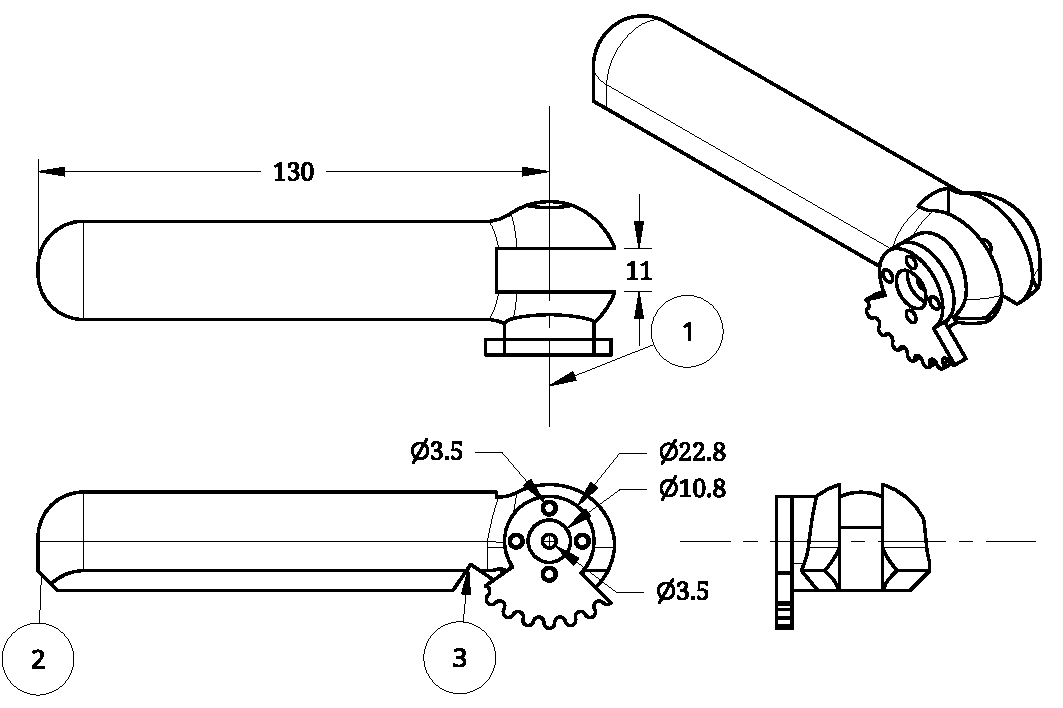
\includegraphics[scale = 0.8]{pics/DrawingC.pdf}
\caption{Illustration of how multiple servo motors are controlled using two timers.}
\label{fig:DrawingC}
\end{figure}

The annotations in Figure \ref{fig:DrawingBase} that shows the base is explained below:
\begin{enumerate}
\item Gear that connects to the servo motor located in leg B.
\item Hole for wire management.
\item Gear teeth that connect to the servo motor located in the base.
\item Centreline where a stainless steel shaft is inserted into bearings for horizontal movement.
\item Centreline where a stainless steel shaft is inserted into bearings for vertical movement.
\end{enumerate}

\begin{figure}[H]
\centering
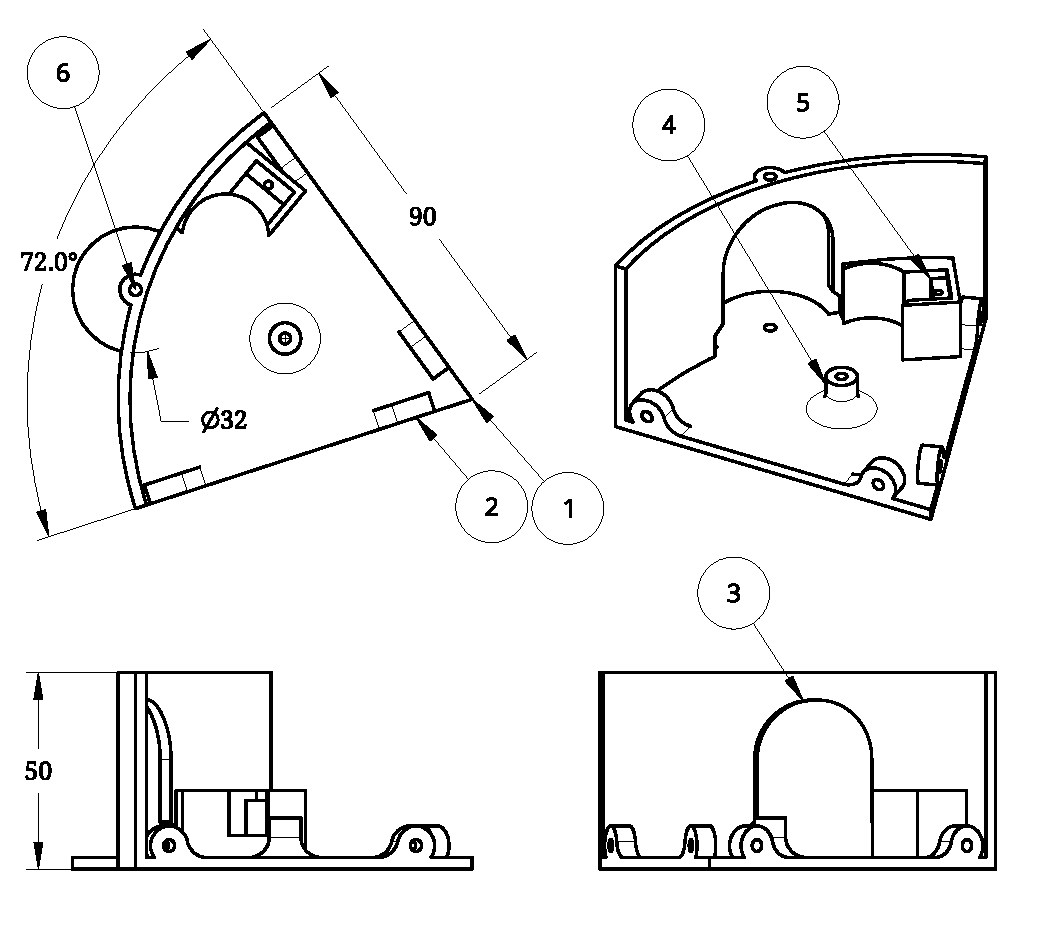
\includegraphics[scale = 0.8]{pics/DrawingBase.pdf}
\caption{Illustration of how multiple servo motors are controlled using two timers.}
\label{fig:DrawingBase}
\end{figure}

\subsubsection{Hardware implementation}

All of the hardware discussed above was 3D printed and assembled.\\

When the hardware was implemented, the servo motors we unable to lift the robot. A spiral torsion spring was designed and printed to help aid the lifting of the robot.\\

The annotations in Figure \ref{fig:DrawingSpring} that shows the torsion spring is explained below:
\begin{enumerate}
\item Hole for stainless steel shaft.
\item Mounting hub on servo gear.
\item Gear for servo.
\end{enumerate}

\begin{figure}[H]
\centering
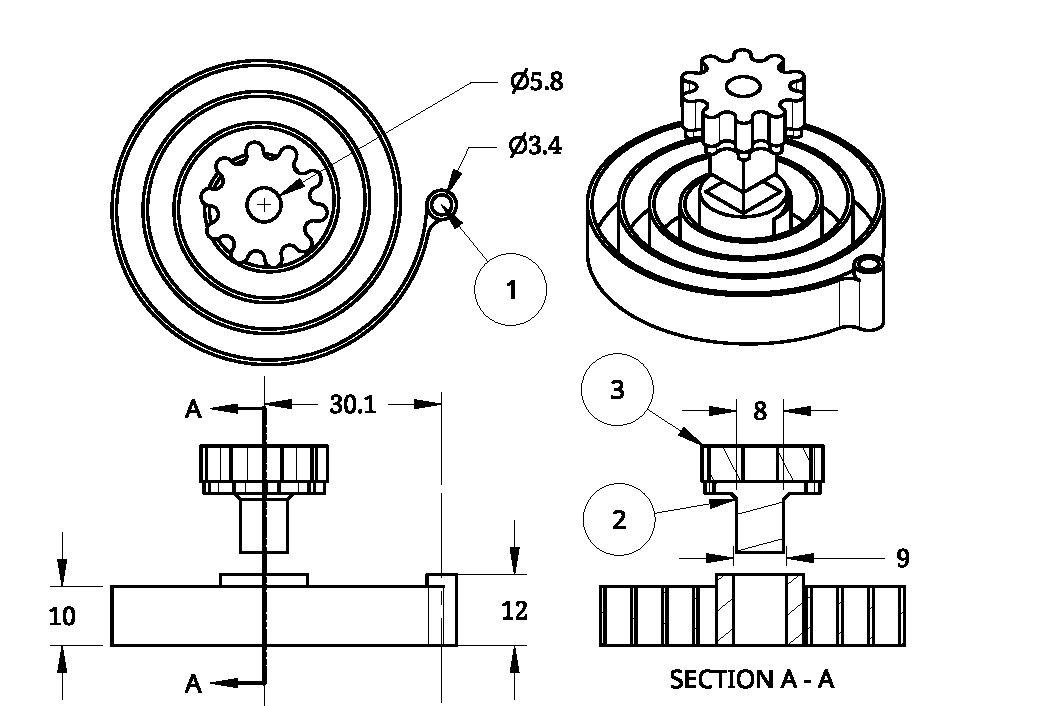
\includegraphics[scale = 0.8]{pics/DrawingSpring.pdf}
\caption{Illustration of how multiple servo motors are controlled using two timers.}
\label{fig:DrawingSpring}
\end{figure}

\subsubsection{Design summary}
\begin{table}[H]
\centering

\begin{tabular}{|p{5cm}|p{5cm}|p{5cm}|}
\hline
\textbf{Task} & \textbf{Implementation} & \textbf{Task complete} \\
\hline
 Development of an IK engine in software & The mathematical analysis of the robot was used to create a generic model, which was then first implemented in Python and thereafter in the final robot implementation. & Completed \\\hline
 
Development of a walking algorithm  & A walking algorithm was developed and optimized in Python and then implemented in the final robot.  & Completed\\\hline

Development of a user interface & The user interface was developed for an Android smartphone using Android Studio. & Completed \\\hline

Communication channel between user interface and robot & Bluetooth was used to establish a low bandwidth, low cost communication system between the smartphone and the robot. It communicates commands successfully. & Completed \\\hline

Implementation of electronics on a PCB.& All electronics were implemented on a Veroboard instead of a PCB which is inexpensive and sufficiently robust for the purpose of this project. A PCB would not have made any functional difference to the end result and is not suited for making changes while prototyping. The only difference would have been aesthetically.& Incomplete \\\hline

Implementation of inclinometer sensor & An inclinometer was planned to give the robot the ability to adapt to the exact angle of slanted surfaces but this was not implemented because the robot walks without a problem on the angles of surfaces specified for this project. & Incomplete \\\hline
\end{tabular}
\caption{Design summary}
\label{my-label}
\end{table}


\secun{Results}

\subsubsection{Summary of results achieved}
\begin{table}[H]
\begin{tabular}{|p{5cm}|p{5cm}|p{5cm}|}
\hline
\textbf{Description of requirement or specification
(intended outcome)} & \textbf{Actual outcome}& \textbf{Location in report}\\
\hline
\multicolumn{3}{|l|}{}\\
\multicolumn{3}{|l|}{\textbf{Mission requirements of the product}}\\
\hline

The robot should be able to move in a given direction in 30 degree increments from a stationary position. & The robot is able to move holonomically, therefore able to move in 30 degree increments.&4.2.1\\\hline

The robot should be able to rotate 90 degrees without translating the centre of the body by more than 5\% of the body diameter.&The robot is able to do this.&4.2.2\\\hline

The time it requires to complete a manoeuvre should not vary more than 25\% between smooth and rough surfaces.&The time differs by about 20\%&4.2.3\\\hline

The robot should be able to walk at a speed of at least 100mm/s.&The robot is only capable of 8mm/s&4.2.4\\\hline

The robot should be able to walk on a surface with a 10\% incline without falling over.&The robot can successfully walk on a slanted surface with an incline of up to 10\% &4.2.5\\\hline

\multicolumn{3}{|l|}{}\\
\multicolumn{3}{|l|}{\textbf{Field conditions}}\\
\hline
The robot should be in range of the wireless smartphone controller.&The robot works fine if it is within a range of 10m of the smartphone&\\\hline

To prevent falling over, the robot should walk on surfaces close to horizontal.&The robot is able to work on slanted surfaces with an incline of less than 10\%&\\\hline

The robot should stay dry to protect electronics.&The robot was never tested in wet conditions&\\\hline

The robot should work in normal temperature conditions for South Africa.&The robot never experienced any issues during the testing phase that relates to ambient temperature, relative humidity or any other atmospheric conditions&\\\hline

\end{tabular}
\caption{Summary of results achieved}
\label{tab:sum}
\end{table}

\subsubsection{Summary of results achieved}
\begin{table}[H]
\begin{tabular}{|p{5cm}|p{5cm}|p{5cm}|}
\hline

\multicolumn{3}{|l|}{}\\
\multicolumn{3}{|l|}{\textbf{Specifications}}\\
\hline
The smartphone application should communicate commands from the user interface to the robot at a frequency of at least 10 Hz.&The smartphone application does do this&\\\hline

The inverse kinematics calculator of the robot should be able to calculate the joint positions correctly to move each leg to the desired location.& This works as designed&\\\hline

The servo motor angles should all be within 5 degrees from the calculated values.& The servo motors are all accurate to within 5 degrees&\\\hline

\multicolumn{3}{|l|}{}\\
\multicolumn{3}{|l|}{\textbf{Deliverables}}\\
\hline
Control code for inverse kinematics and servo control.&This was completed and is functional&\\\hline

Android application with a user interface for control of the robot.&This was completed and is functional&\\\hline

Circuits implemented on PCB for interfacing all hardware with the microcontroller.&This was performed on Veroboard instead of PCB&\\\hline

Robot body and legs.& This was all successfully 3D printed&\\\hline

Simulations on all implemented software and analogue design& Tis was completed and is functional&\\\hline

\end{tabular}
\caption{Summary of results achieved (continued)}
\label{tab:sum2}
\end{table}

\subsubsection{Qualification tests}

%Test 1
\paragraph{Qualification test \arabic{paragraph} : Holonomic translation}
\label{par:1}
\subparagraph{Qualification test}
\textit{Objectives of test/experiment}\\
The objective is to prove that the robot is capable of moving in any direction from a standing position without first rotating.
\textit{Equipment used}\\
A canvas with lines in 30 degree increments is used to put the robot on.
\textit{Experimental parameters and setup }\\
The robot is turned on and placed in the centre of the canvas. The test is conducted in the field conditions listed in Table \ref{tab:sum}.
\textit{Experimental protocol}\\
The robot is instructed to move along one of the lines and then return to the centre by using the smartphone as remote control. Once back in the centre, the next line is followed. This process continues until all the lines have been followed.
\subparagraph{Results and observations}
\textit{Measurements}\\
Figure \ref{fig:Res1} shows the robot on the canvas where the qualification test is being performed.
\begin{figure}[H]
\centering
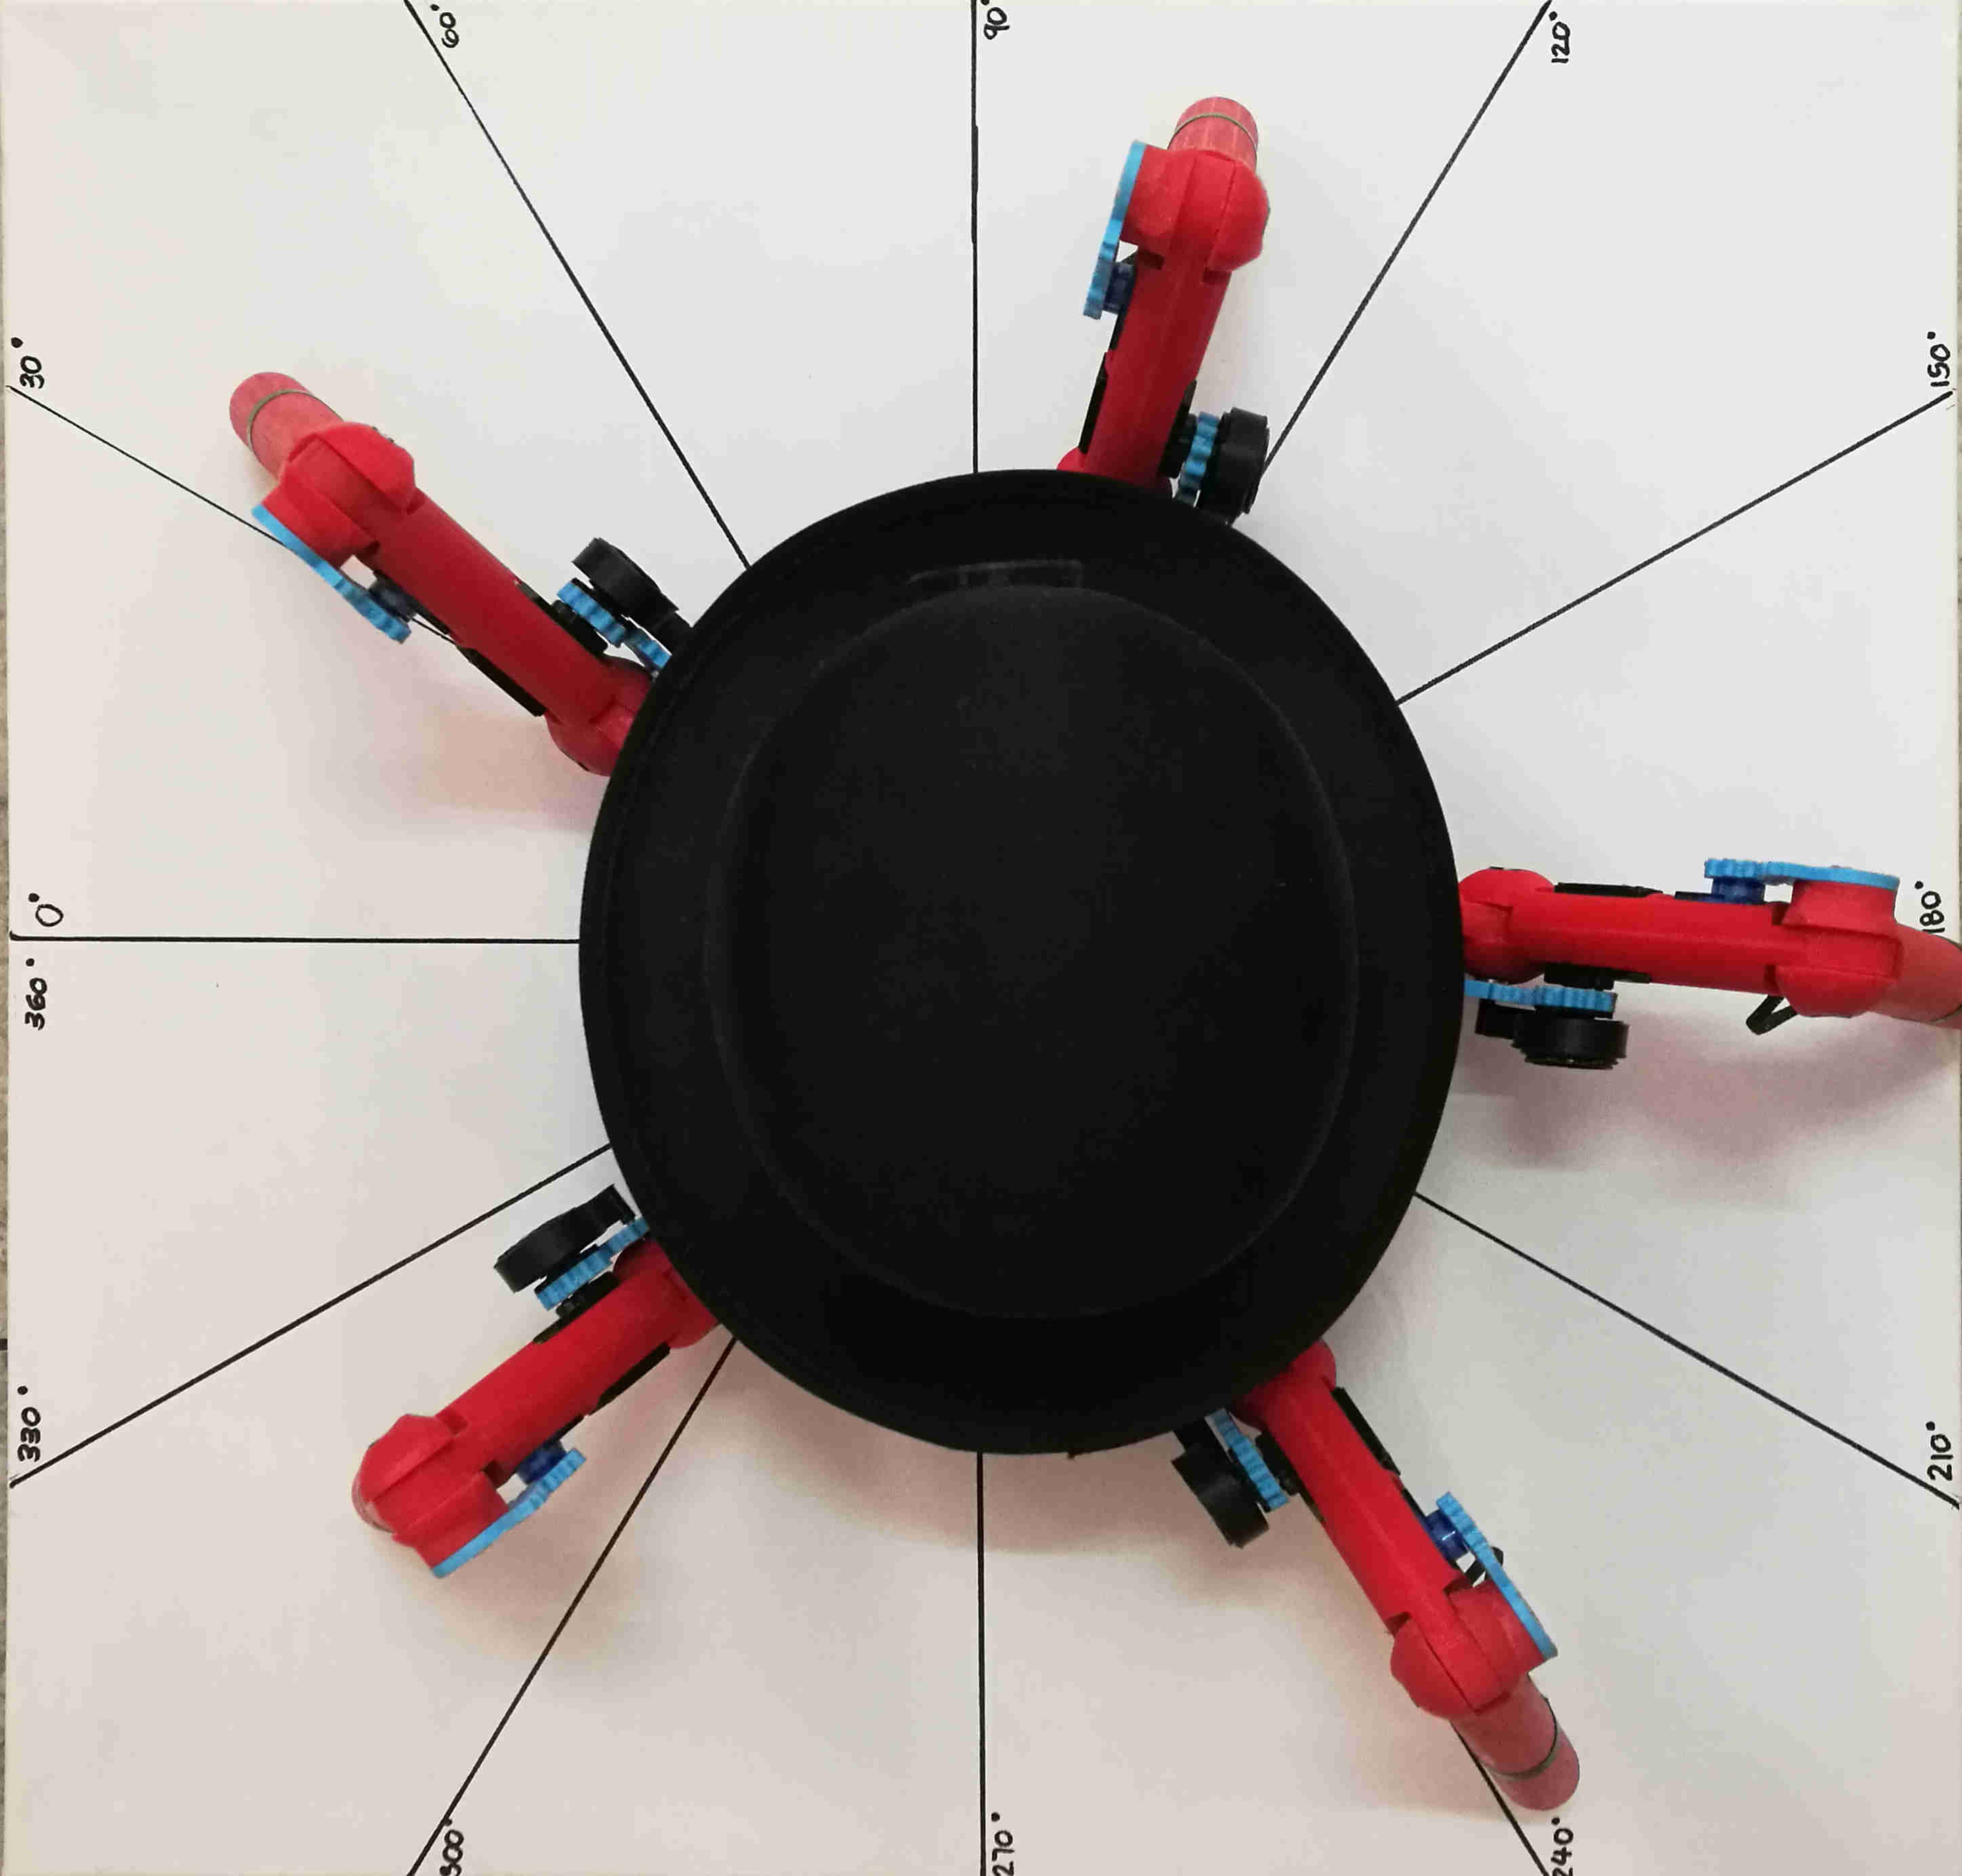
\includegraphics[scale = 1]{pics/Res1.jpg}
\caption{Top view of the robot on the canvas.}
\label{fig:Res1}
\end{figure}
\textit{Description of results}\\
The robot is able to successfully follow the lines on the canvas without ever rotating.

%Test 2
\paragraph{Qualification test \arabic{paragraph} : Rotation without translation}
\subparagraph{Qualification test}
\textit{Objectives of test/experiment}\\
The objective of this test is to confirm that the robot is capable of rotating around its own axis without translating.
\textit{Equipment used}\\
The same canvas used in \ref{par:1} is used for this qualification test. It has two circles, one has the diameter of the robot base, the second is 5\% larger.
\begin{figure}[H]
\centering
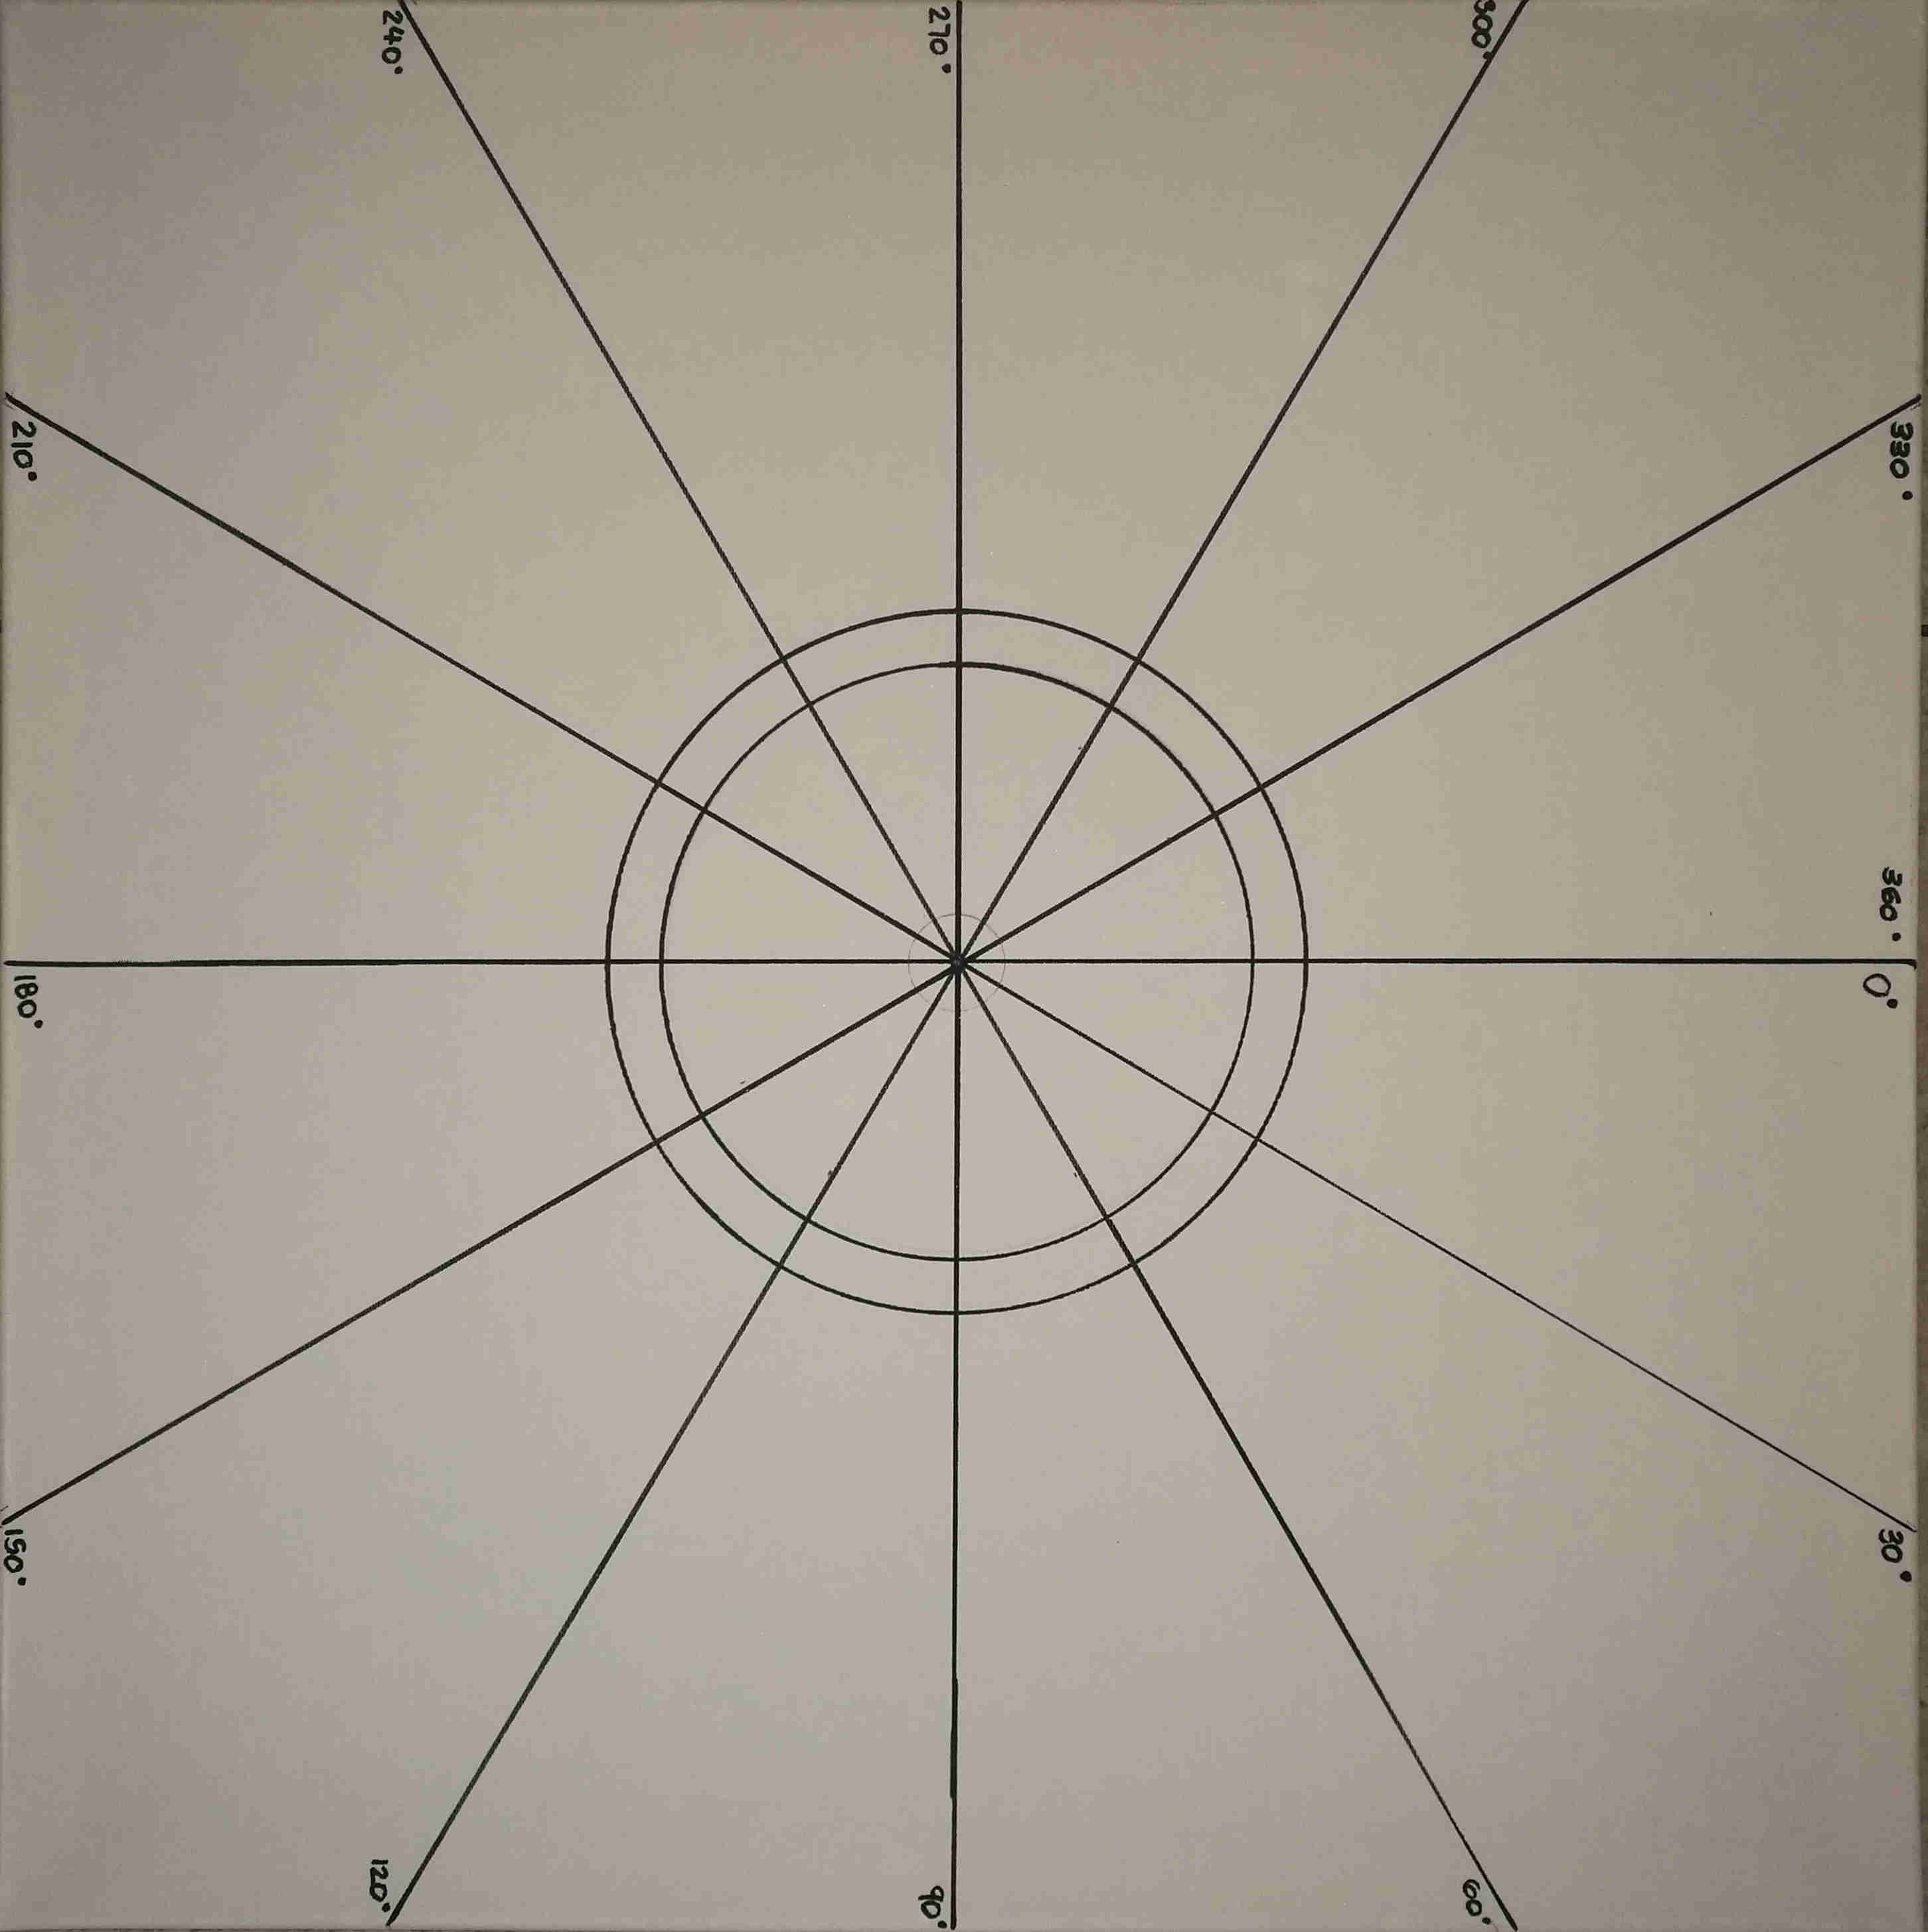
\includegraphics[scale = 1]{pics/Res2.jpg}
\caption{Canvas used for this experiment.}
\label{fig:Res2}
\end{figure}
\textit{Experimental parameters and setup }\\
The robot is placed inside the smaller circle and switched on. The test is conducted in the field conditions listed in Table \ref{tab:sum}.
\textit{Experimental protocol}\\
The robot is instructed to rotate from the smartphone application. After 90 degrees of rotation, the robot is instructed to stop and is then turned off. The robot should be within the bigger circle.
\subparagraph{Results and observations}
\textit{Measurements}\\
\begin{figure}[H]
\centering
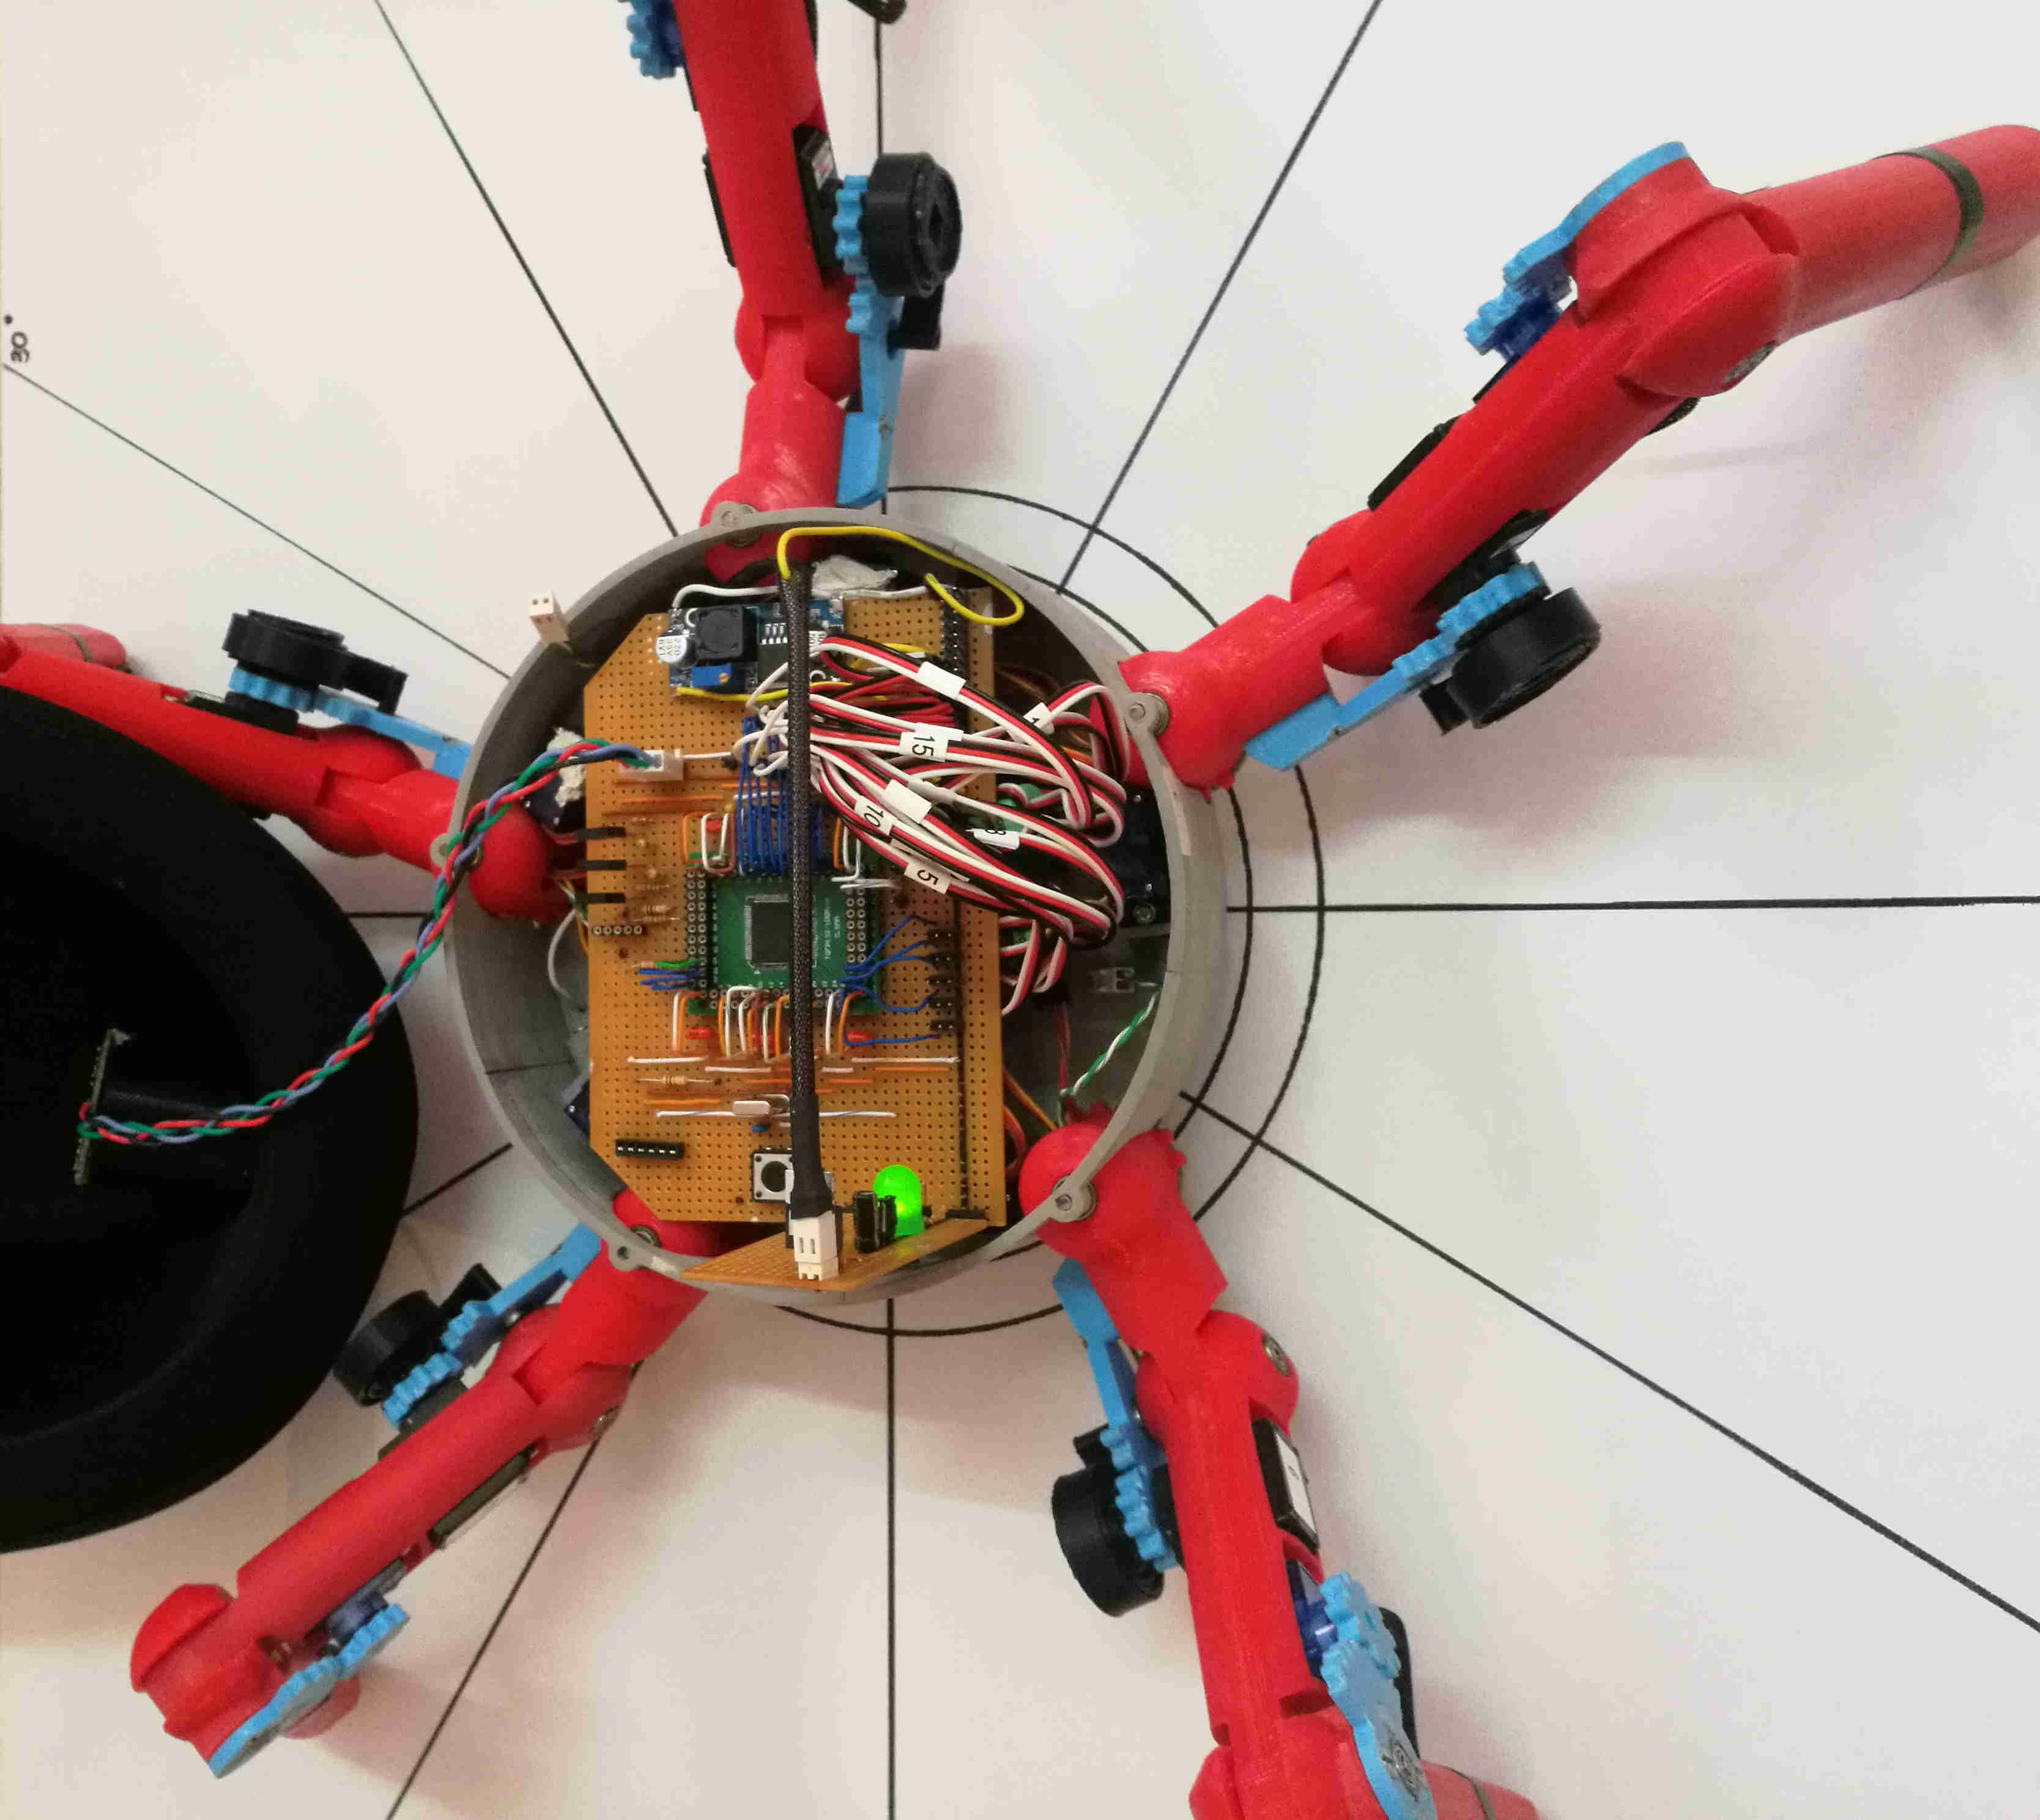
\includegraphics[scale = 1]{pics/Res3.jpg}
\caption{Robot inside the larger circle}
\label{fig:Res3}
\end{figure}
\textit{Description of results}\\
The robot is still inside the larger circle after rotating 90 degrees.

%Test 3
\paragraph{Qualification test \arabic{paragraph} :Speed on rough terrain}
\subparagraph{Qualification test}

\textit{Objectives of test/experiment}\\The purpose of this test is to show that the robot functions reasonably well on rough terrain when compared to a smooth surface.
\textit{Equipment used}\\
A small test track developed for this purpose is used. In order to compare performance between the smooth and rough terrain, the time to complete the track is recorded with a stopwatch application on a smartphone.
\textit{Experimental parameters and setup }\\
A rough terrain is simulated by scattering small, loose obstacles (foam blocks) over the test track. This is a realistic representation of a wide variety of terrain conditions. For preparation the robot is placed on the start line of the smooth test track and switched on. The test is conducted in the field conditions listed in Table \ref{tab:sum}.
\textit{Experimental protocol}\\
The stopwatch is started and the robot is instructed to follow the line that forms the test track. When the robot reaches the end, the time on the stopwatch is recorded. The test track is scattered with the small obstacles and the procedure is repeated.
\begin{figure}[H]
    \centering
    \begin{subfigure}[t]{0.5\textwidth}
        \centering
        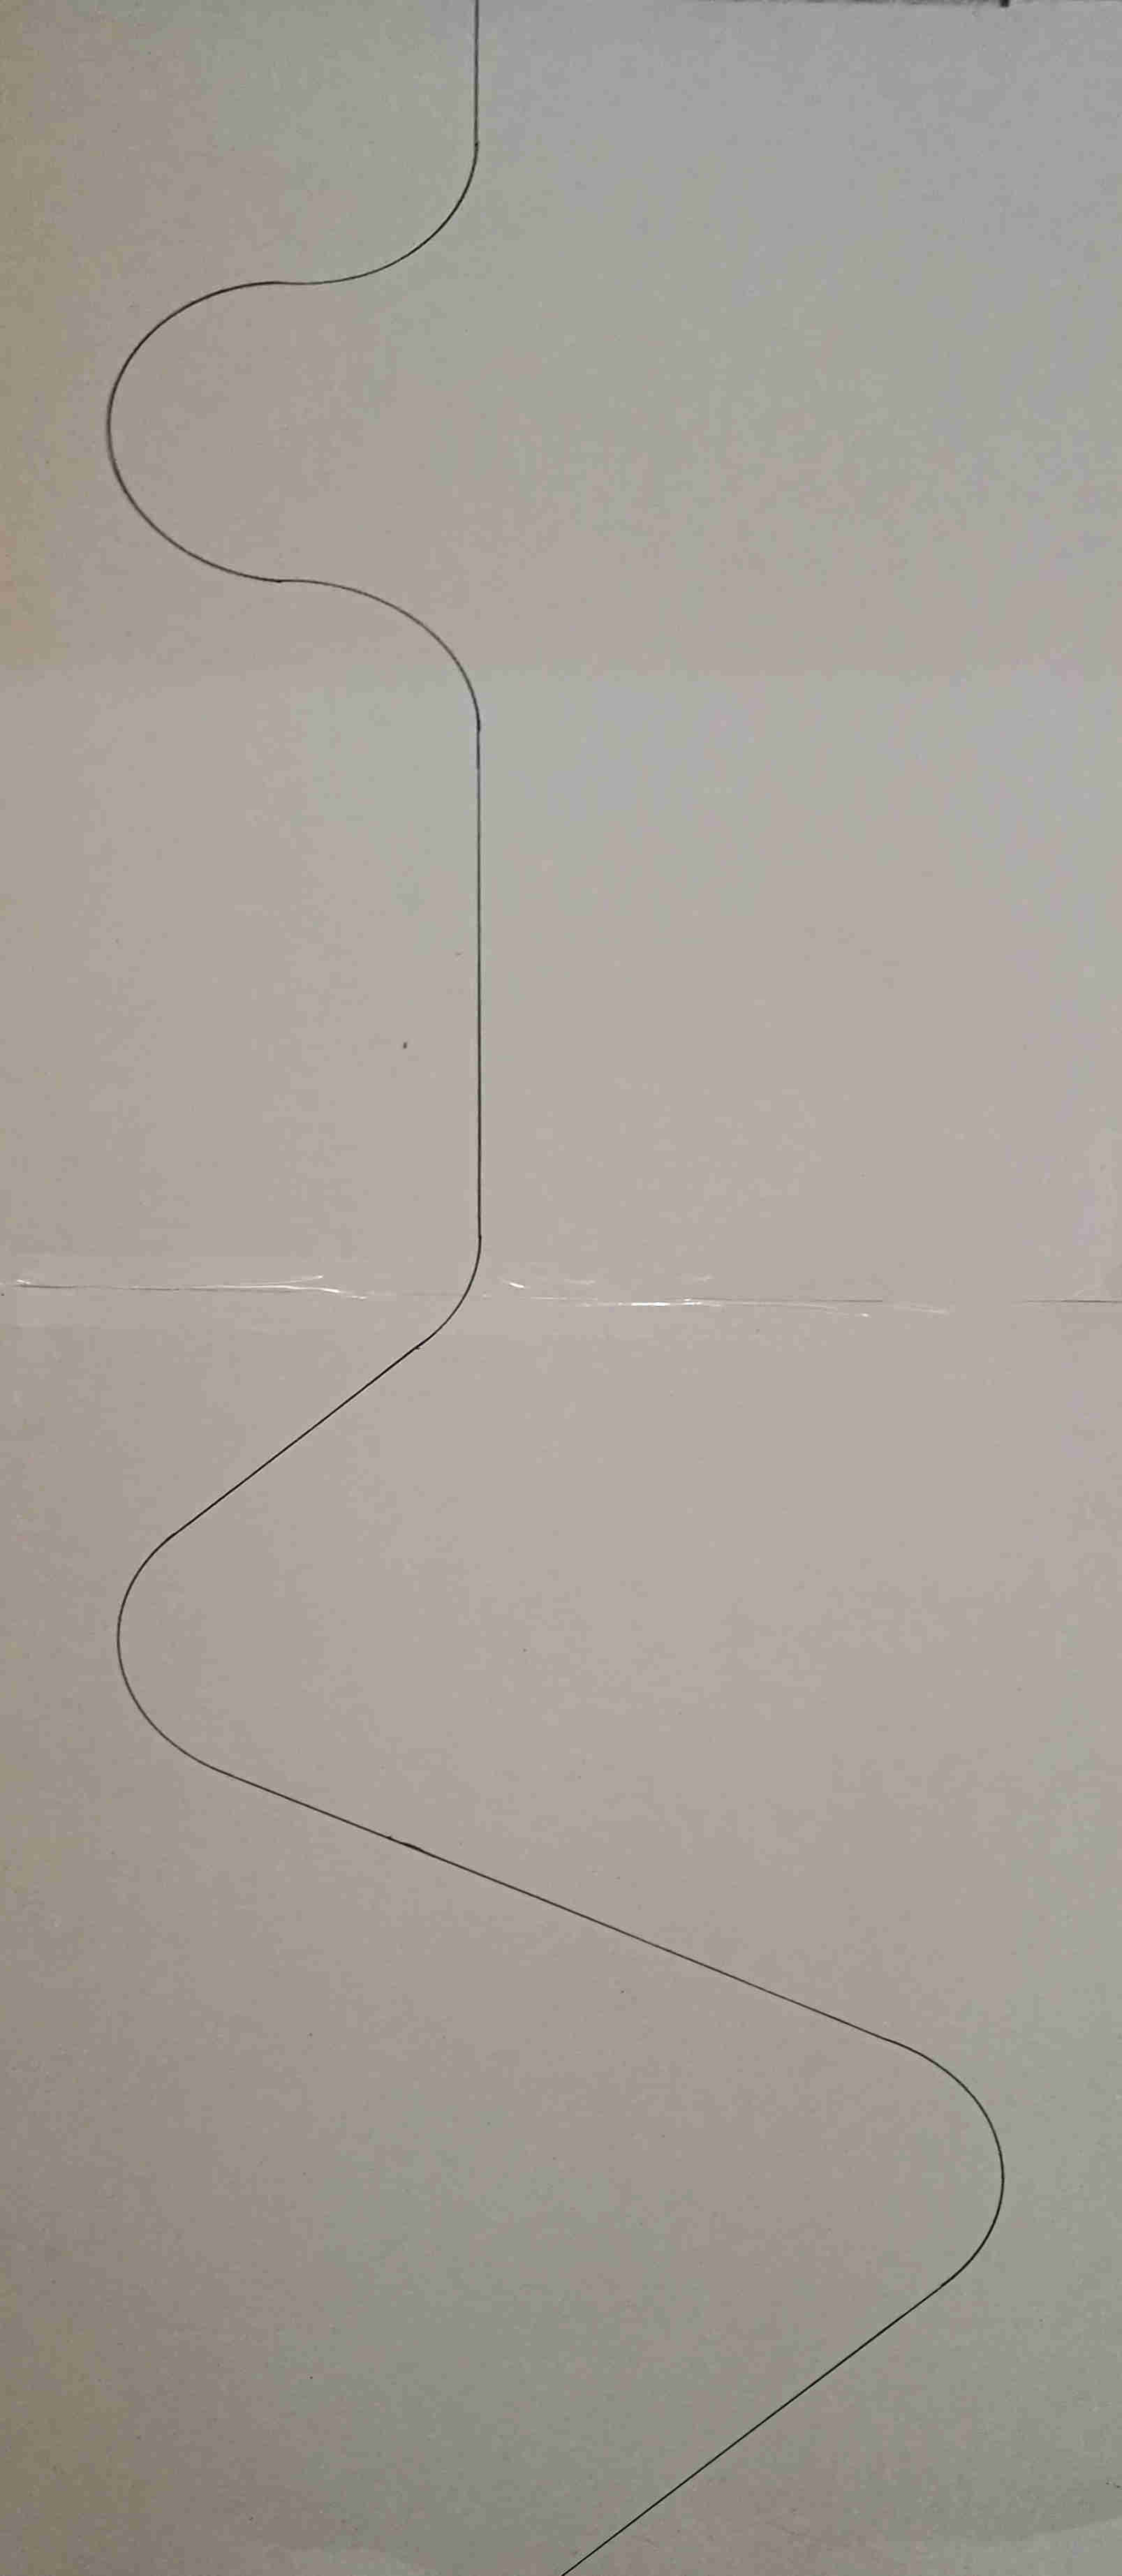
\includegraphics[scale = 1]{pics/Res5.jpg}
        \caption{Test track without obstacles.}
    \end{subfigure}%
    ~ 
    \begin{subfigure}[t]{0.5\textwidth}
        \centering
        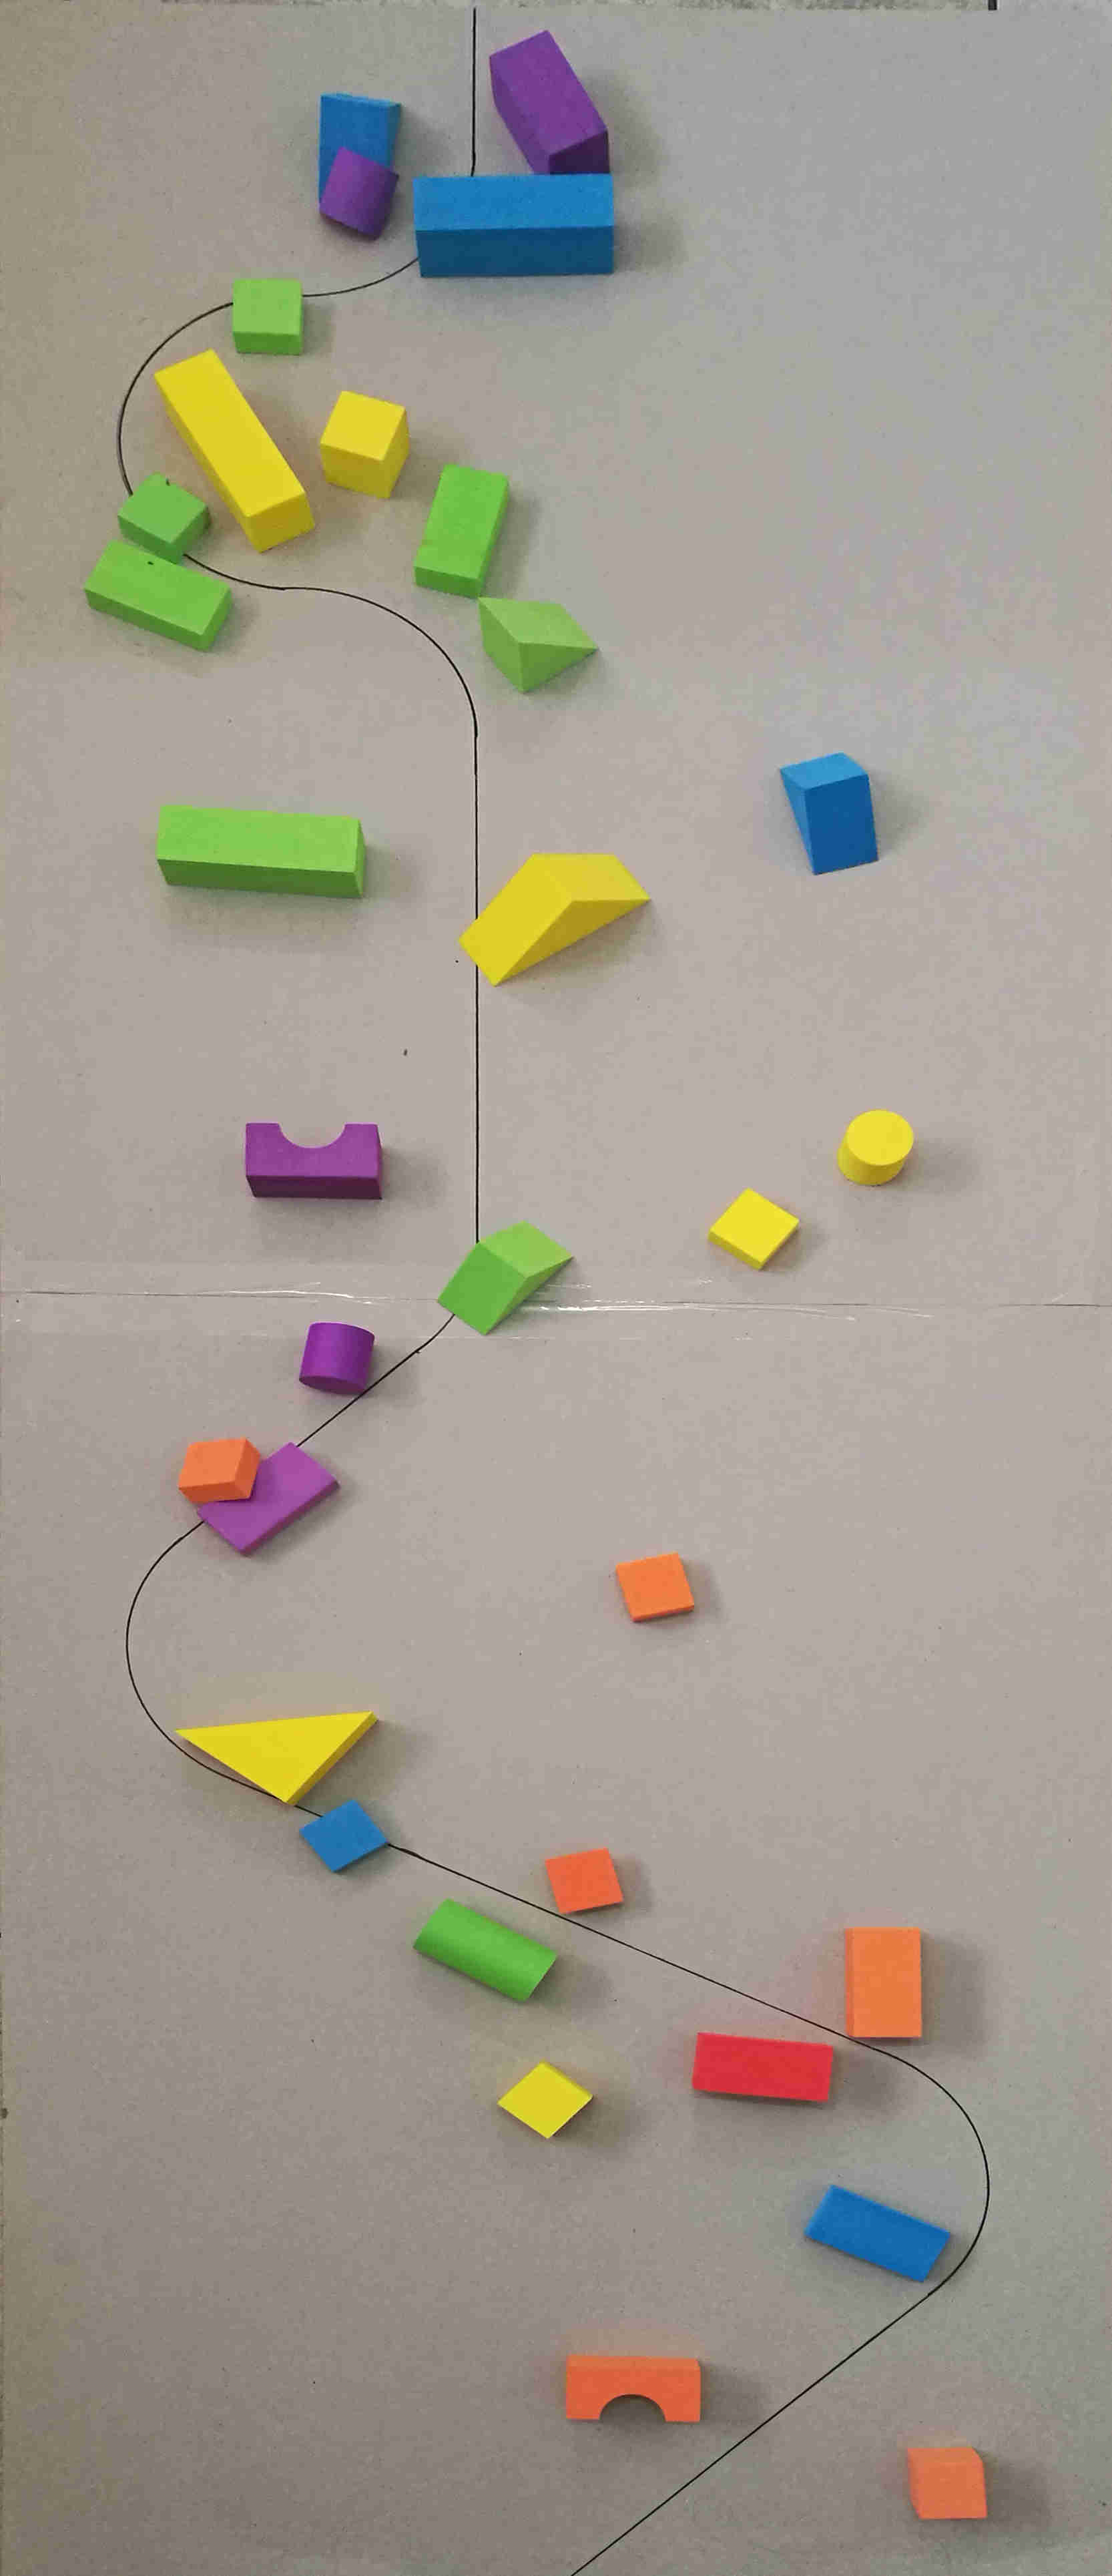
\includegraphics[scale = 1]{pics/Res4.jpg}
        \caption{Test track with obstacles.}
    \end{subfigure}
    \caption{Test setup for proving that the robot can easily walk on rough surfaces}
    \label{fig:Res4}
\end{figure}
Figure \ref{fig:Res4} shows the test track for the two different tests.
\subparagraph{Results and observations}
\textit{Measurements}\\
\begin{table}[H]
\centering
\begin{tabular}{|l|l|}
\hline
\textbf{Course condition}&\textbf{Time}\\\hline
Smooth&5:12\\\hline
Rough & 6:20\\
\hline
\end{tabular}
\caption{Results achieved for the test track}
\label{my-label}
\end{table}
\textit{Description of results}\\
The robot moves slower over the obstacles than on the smooth course.

%Test 4
\paragraph{Qualification test \arabic{paragraph} : Speed}
\subparagraph{Qualification test}
\textit{Objectives of test/experiment}\\
The objective of this test is to prove that the robot can reach a speed of 100mm/s
\textit{Equipment used}\\
A linear track designed for this experiment is used to measure the speed. It has markings that is a fixed distance apart that makes it easy to measure the distance travelled. The time will be recorded using a stopwatch application on a smartphone. 
\begin{figure}[H]
\centering
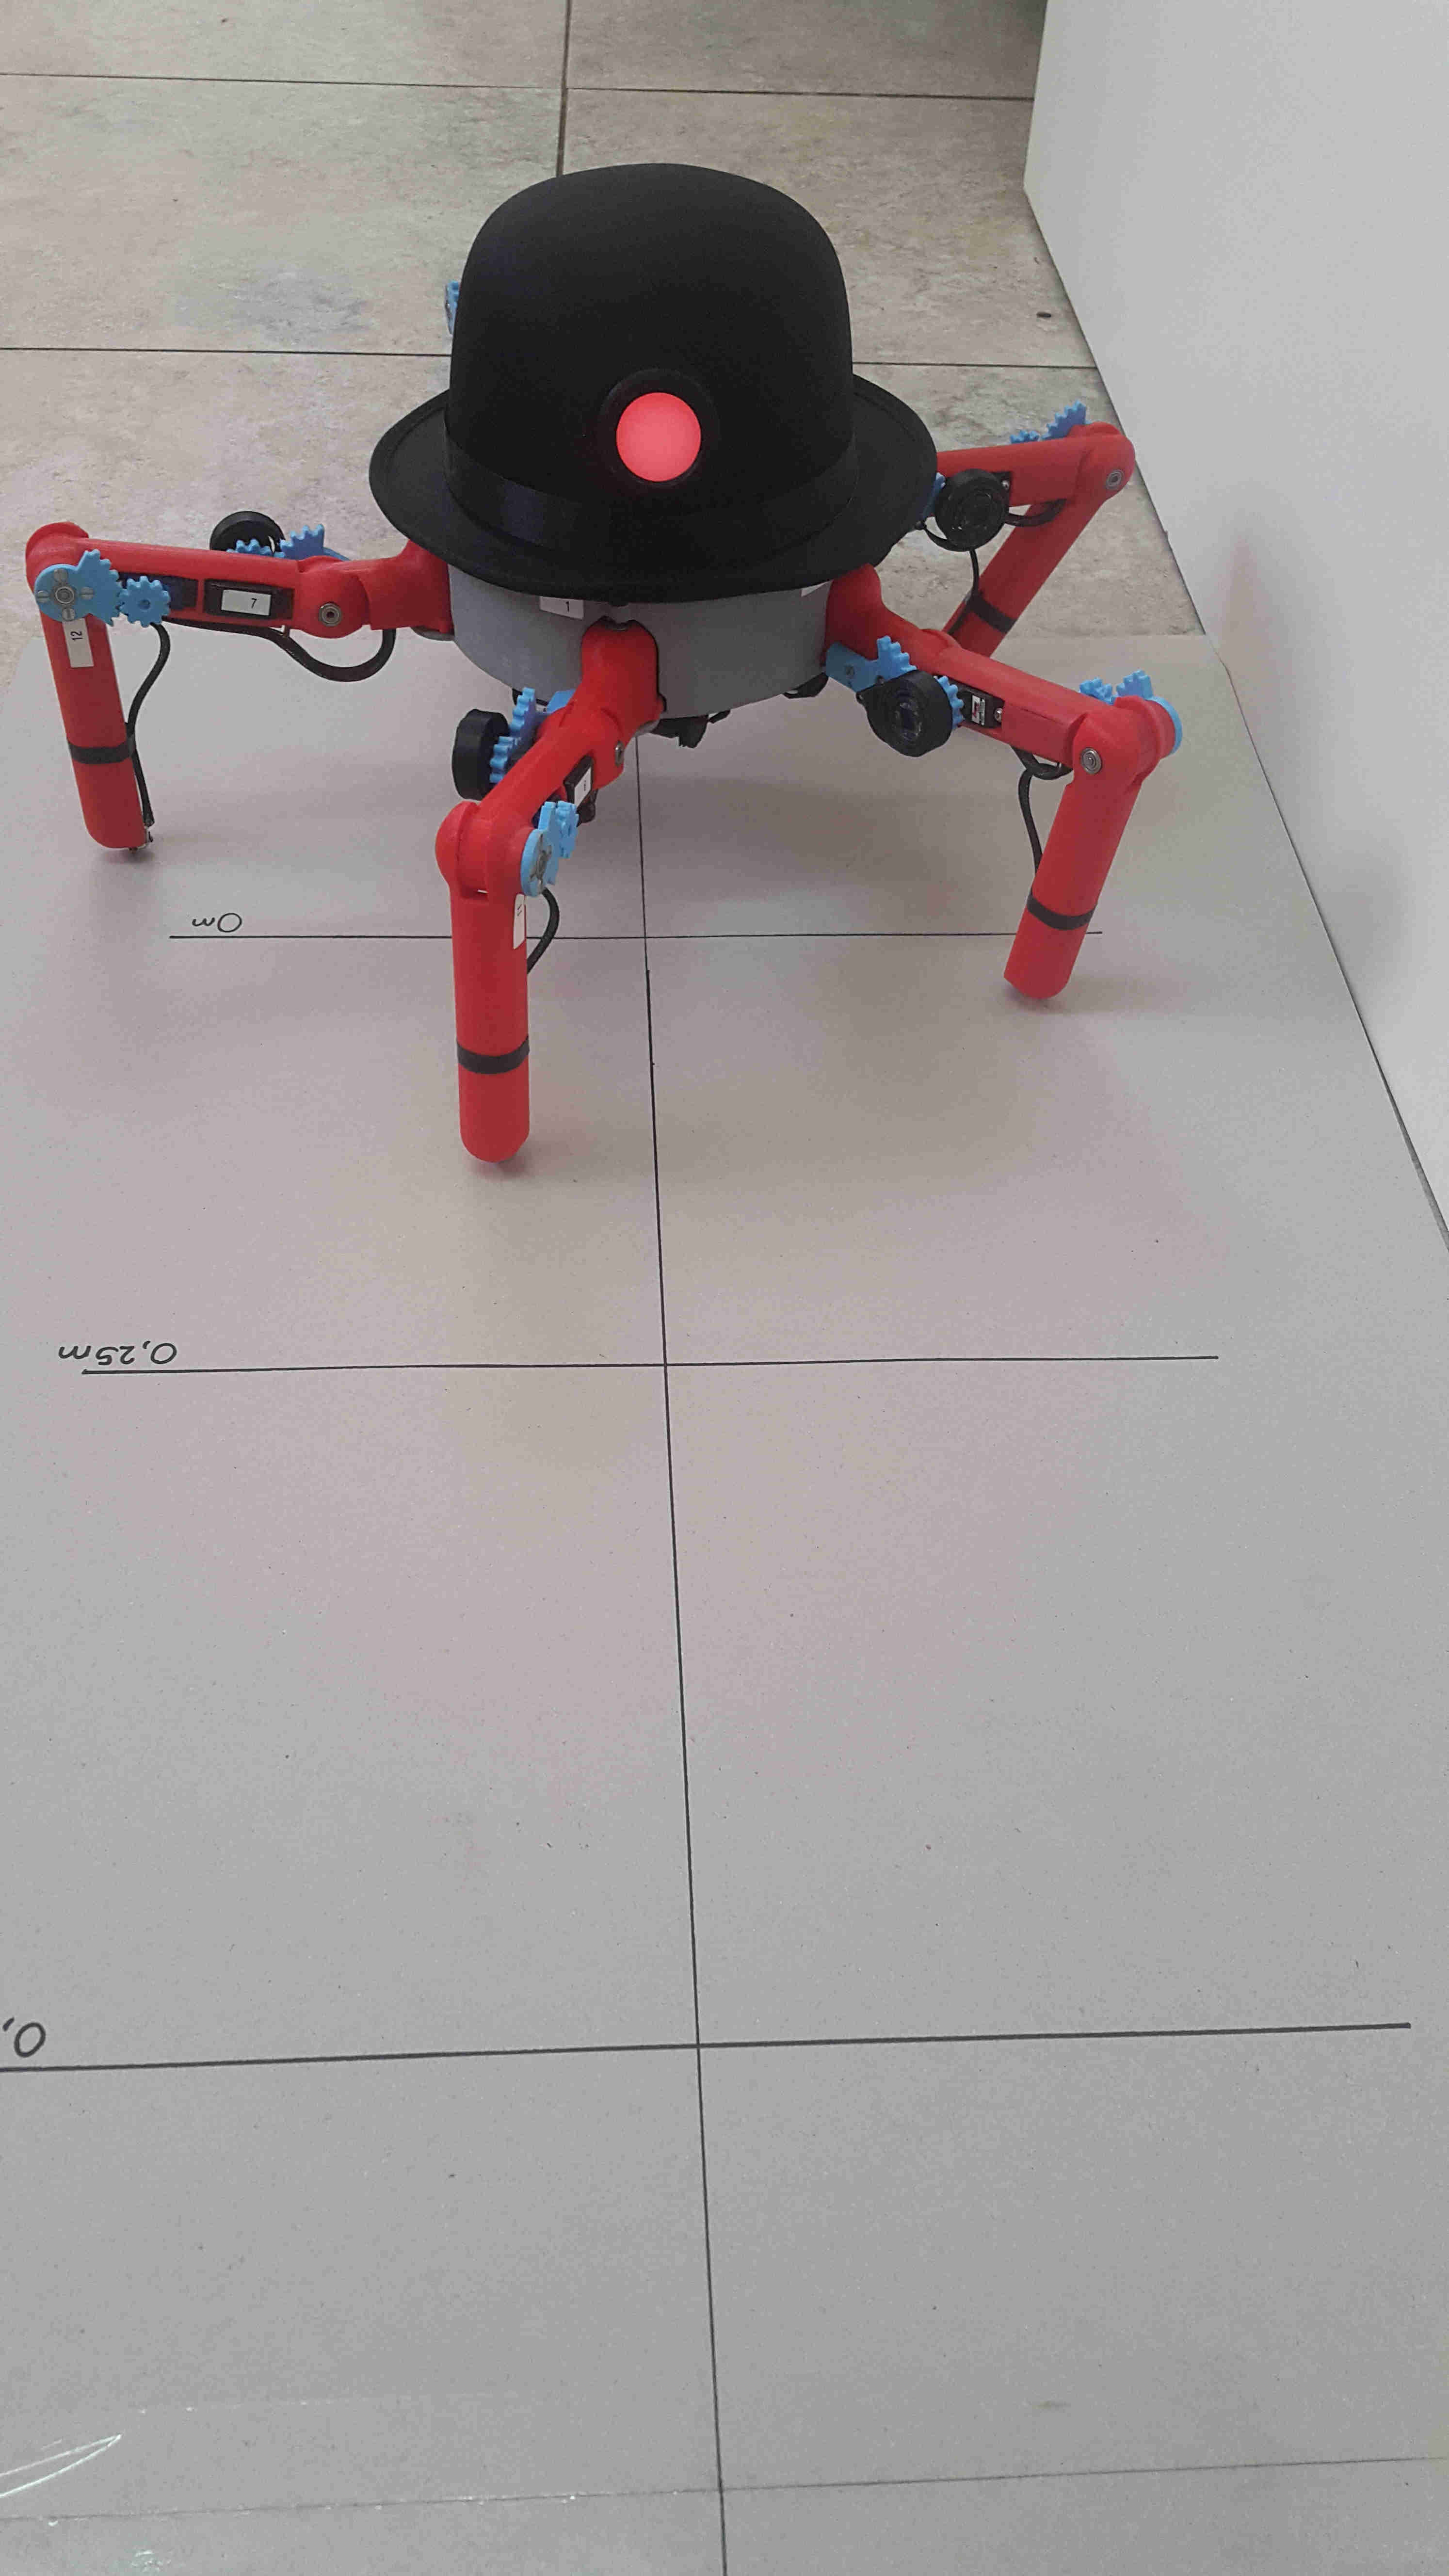
\includegraphics[scale = 1]{pics/Res6.jpg}
\caption{Robot on the track for measuring speed.}
\label{fig:Res6}
\end{figure}
Figure \ref{fig:Res6} shows the robot on the track mentioned above.
\textit{Experimental parameters and setup }\\
The robot is placed at the start of the track and switched on. The test is conducted in the field conditions listed in Table \ref{tab:sum}.
\textit{Experimental protocol}\\
The stopwatch is started and the robot is instructed to move down the track as fast as possible. When the end of the track is reached, the time on the stopwatch is recorded.
\subparagraph{Results and observations}
\textit{Measurements}\\
\begin{table}[H]
\centering
\begin{tabular}{|l|l|l|}
\hline
\textbf{Distance}&\textbf{Time}&\textbf{Speed}\\\hline
1.5m&3:07&8mm/s\\\hline
\end{tabular}
\caption{Results achieved for the speed test track}
\label{my-label}
\end{table}
\textit{Description of results}\\
The robot moves much slower than anticipated.

%Test 5
\paragraph{Qualification test \arabic{paragraph} :Slopes}
\subparagraph{Qualification test}
\textit{Objectives of test/experiment}\\
The objective is to prove that the robot is capable of walking on a slanted surface without falling over.
\textit{Equipment used}\\
A plank is used to create the slanted surface. A long ruler is used to measure the incline of the plank.
\textit{Experimental parameters and setup }\\
The plank is angled at 10\%. This is ensured by making sure that the plank has a height of 10cm at the point that is 1m from the edge of the plank on the ground. The robot is put at the base of the plank. The test is conducted in the field conditions listed in Table \ref{tab:sum}.
\textit{Experimental protocol}\\
The robot is instructed to walk on the plank to see if it struggles or falls over at any stage in the process.
\subparagraph{Results and observations}
\textit{Description of results}\\
The robot walks without any additional difficulty due to the incline. The robot was never close to falling over at any stage in the experiment.

%Test 6
\paragraph{Qualification test \arabic{paragraph} :Slippery surfaces}
\subparagraph{Qualification test}
\textit{Objectives of test/experiment}\\
The objective is investigate the performance of the robot on a slippery surface
\textit{Equipment used}\\
A wooden floor is used as the slippery surface for the robot to walk on.
\textit{Experimental parameters and setup }\\
The robot is put on the wooden floor and turned on. The test is conducted in the field conditions listed in Table \ref{tab:sum}.
\textit{Experimental protocol}\\
The robot is instructed to walk on the wooden floor in both slow and rapid movements to investigate how the legged design functions on low traction environments.
\subparagraph{Results and observations}
\textit{Description of results}\\
The robot with more difficulty on slippery surfaces than on surfaces withh higher traction.

\secun{Discussion}
\newpage
\subsubsection{Interpretation of results}
The results recorded in the previous section of this report indicate that the robot is able to function as a holonomic robot, therefore it is able to move in any direction without first rotating and rotate without translating. The results that measure the performance of the robot, however, show that it does not do it nearly as good as it was designed to do it. The maximum speed of the robot, for example, is far below what was aimed for originally. The fact that the robot is able to correctly execute commands shows that the theoretical design and algorithm is valid. In the case of the speed requirement, it is the mechanical design that was lacking. The robot was far heavier that planned for and the servo motors used struggle to carry the load. The only way to make the robot function is to slow all of the movements down. The test on slippery surfaces had unexpected results as well. The expectation was that the robot might struggle to walk because the legs would slip on the floor and it would slip when propelling itself forward. Instead the low friction causes the legs to want to spread outwards, causing more strain on the servo motors. The choice of servo motor implemented in the robot caused the robot to not work as good as it should have. If more powerful servo motors were implemented, the power consumption would have been significantly higher but torque would have been sufficient.  

\subsubsection{Aspects to be improved}
The mechanical drive system for the legs could be improved. Torque at the critical joint is not sufficient and the full range of motion is not used. A solution that would not require a complete redesign would be to change the gear ratio at the critical joint to have a more powerful actuator with a smaller range of motion

\subsubsection{Strong points}

\subsubsection{Under which circumstances will the current system fail?}

\subsubsection{Design ergonomics}

\subsubsection{Health and safety aspects of the design}

\subsubsection{Social and legal impact and benefits of the design}

\subsubsection{Environmental impact and benefits of the design}

\secun{Conclusion}
\subsubsection{Summary of the work}
The mathematical analysis of the generic robot body was done in such a way that the model could be changed parametrically to allow for greater flexibility in the design process. This was applied and developed in a Python simulation which eventually ended up to include a user interface and a plot of the robot body in action. Once the walking algorithm was implemented and optimized, the work was implemented in C to be used in the microcontroller that would control the robot. Algorithms were designed and implemented to control all 15 of the servo motors with as little hardware and software resources required as possible. An android application was developed to be a user interface and act as a remote control for the robot. Instructions are sent to the robot using Bluetooth, which are received by a Bluetooth module connected to the microcontroller with a serial connection. Legs and a body was 3D-printed to fit the servo motors and the robot was able to move its first legs. The movement of legged vehicles on slippery surfaces was investigated and the results were surprising. The investigation was somewhat limited by the available torque from the servo motors.\\
\subsubsection{Summary of the observations and findings}
The robot is able to walk but not in the way originally intended. Although holonomic motion is possible and those design goals have been met, the robot struggles to move properly. This is a result of the robot being much heavier than anticipated. The extra strain on the servo motors causes a high power demand from the servo motors which the DC-DC converter is not always able to supply. The result in the rail voltage is that dips occur when the robot requires strength for more than one leg at a time. The dip in voltage reduces the servo torque, making the situation even worse. A partial solution to this is to keep the robot as light as possible and severely limit the speed of all movements. This somewhat helps but the robot is no longer able to meet the mission critical specification for speed. The movement accuracy also suffers from the same problem.\\
\subsubsection{Suggestions for future work}
The work could be continued and largely improved by getting the robot to walk properly without exchanging the servo motors with stronger ones. This could possibly be done by changing the gear ratio on the outer two limbs to sacrifice some range for torque. This will allow the design to keep the low power consumption it was aiming for while being able to work as intended in the design.

